% Vorlage für eine Bachelorarbeit
% Siehe auch LaTeX-Kurs von Mathematik-Online
% www.mathematik-online.org/kurse
% Anpassungen für die Fakultät für Mathematik
% am KIT durch Klaus Spitzmüller und Roland Schnaubelt Dezember 2011

\documentclass[12pt,a4paper]{scrartcl}

% scrartcl ist eine abgeleitete Artikel-Klasse im Koma-Skript
% zur Kontrolle des Umbruchs Klassenoption draft verwenden


% die folgenden Packete erlauben den Gebrauch von Umlauten und ß
% in der Latex Datei
\usepackage[utf8]{inputenc}
% \usepackage[latin1]{inputenc} %  Alternativ unter Windows
\usepackage[T1]{fontenc}
\usepackage[ngerman]{babel}


\usepackage[pdftex]{graphicx}
\usepackage{latexsym}
\usepackage{amsmath,amssymb,amsthm}
\usepackage{mathtools}
\usepackage{ae,aecompl}
\usepackage{blindtext}
\setcounter{secnumdepth}{5}
\usepackage{graphicx}
\graphicspath{ {./images/} }
\usepackage{hyperref}
\usepackage{acronym}
\usepackage{subcaption}
\usepackage[dvipsnames]{xcolor}
\usepackage{tikz}
\usepackage{tkz-euclide}
\usepackage{pgfplots}
\usetikzlibrary{matrix, positioning}

\usetikzlibrary{arrows,automata, matrix,chains,positioning,decorations.pathreplacing,arrows}

% Abstand obere Blattkante zur Kopfzeile ist 2.54cm - 15mm
\setlength{\topmargin}{-15mm}


\numberwithin{equation}{section} 

% einige Abkuerzungen
\newcommand{\C}{\mathbb{C}} % komplexe
\newcommand{\K}{\mathbb{K}} % komplexe
\newcommand{\R}{\mathbb{R}} % reelle
\newcommand{\Q}{\mathbb{Q}} % rationale
\newcommand{\Z}{\mathbb{Z}} % ganze
\newcommand{\N}{\mathbb{N}} % natuerliche



\begin{document}
  % Keine Seitenzahlen im Vorspann
  \pagestyle{empty}

  % Titelblatt der Arbeit
  \begin{titlepage}

    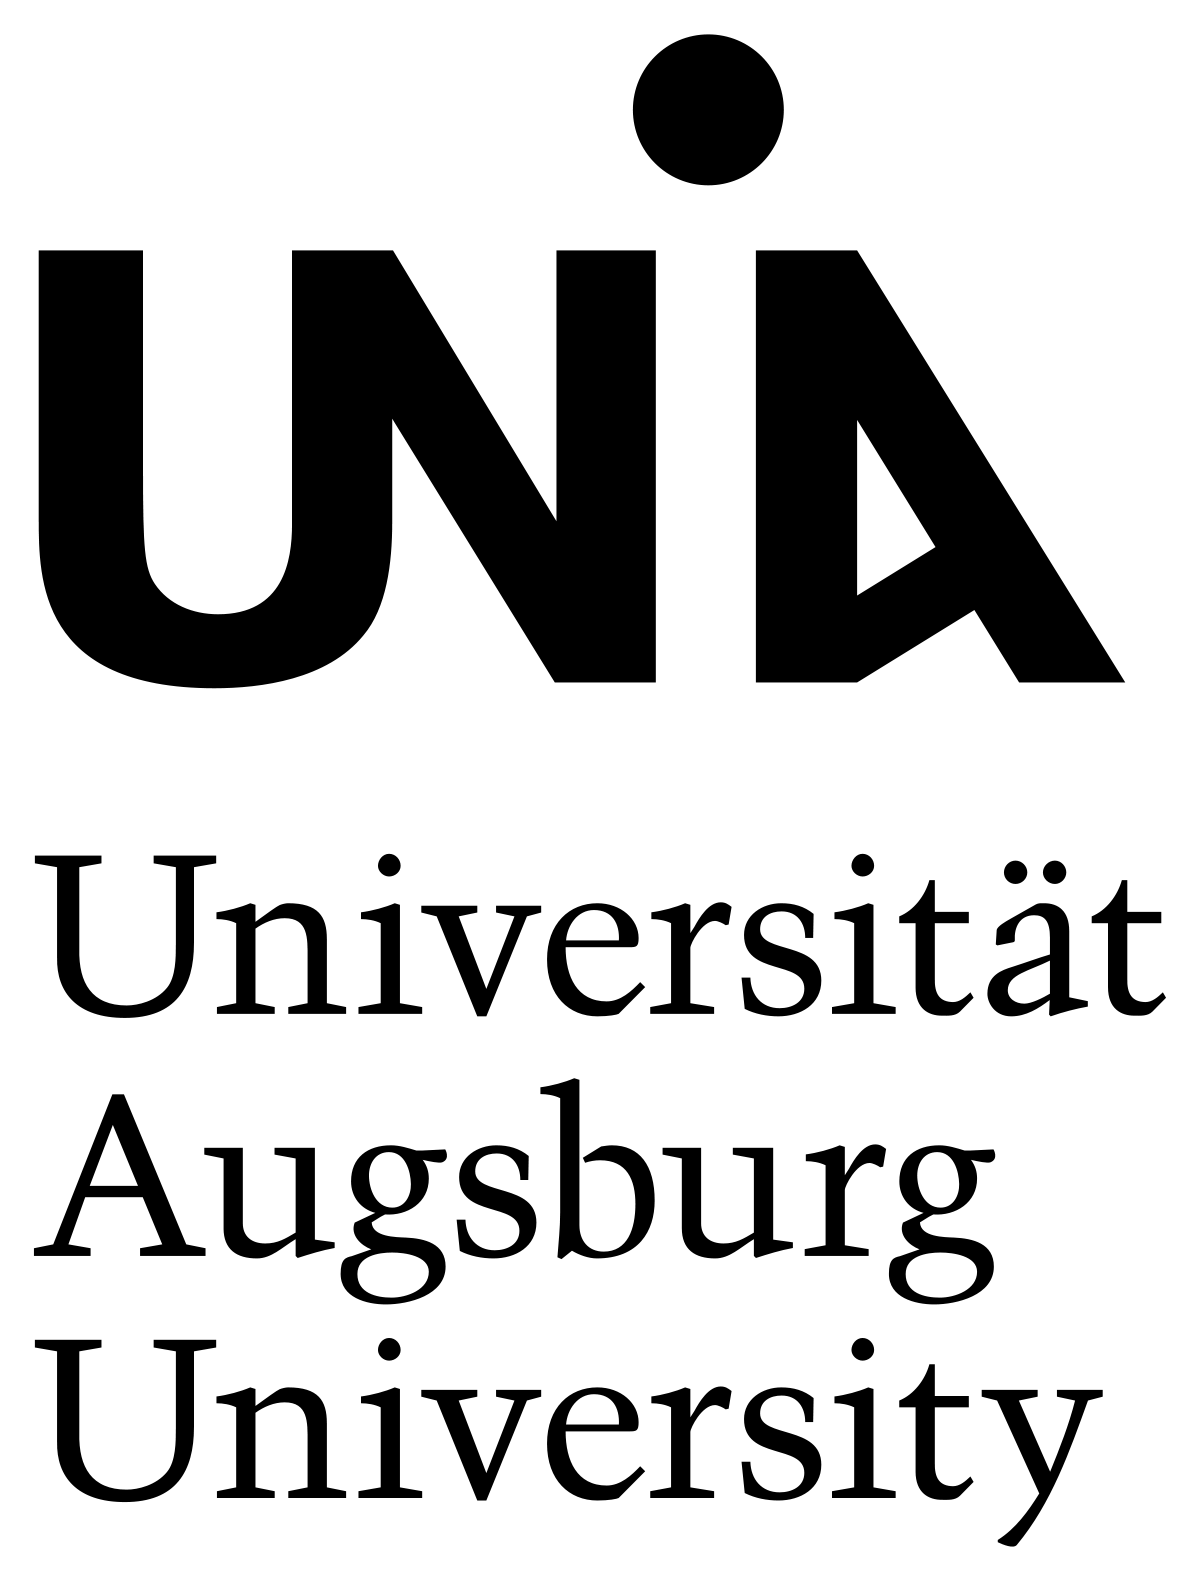
\includegraphics[scale=0.05]{logo_uni} 
    \vspace*{2cm} 

 \begin{center} \large 
    
    Bachelorarbeit
    \vspace*{2cm}

    {\huge Titel der Bachelorarbeit: Image Analysis for Food Safety and Health}
    \vspace*{2.5cm}

    Name des Autors: TEMKENG Thibaut
    \vspace*{1.5cm}

    Datum der Abgabe: Ende Oktober
    \vspace*{4.5cm}


    Betreuung: Name der Betreuer/ des Betreuers:Shou Liu \\[1cm]
    Fakultät für Embedded Intelligence for Health Care and Wellbeing \\[1cm]
%		Karlsruher Institut für Technologie
  \end{center}
\end{titlepage}



  % Inhaltsverzeichnis
  \tableofcontents
  \listoffigures

\newpage
 


  % Ab sofort Seitenzahlen in der Kopfzeile anzeigen
  \pagestyle{headings}

\section{Einleitung}



%%%%%%%%%%%%%%%%%%%%%%%%%%%%%%%%%
 \newpage  % neuer Abschnitt auf neue Seite, kann auch entfallen
%%%%%%%%%%%%%%%%%%%%%%%%%%%%%%%%%
 
\section{Grundlagen}
\subsection{Entwicklung von Künstlichen Neuronalen Netzen }

\paragraph{künstliches Neuron}.\\
Ein künstliches Neuron\cite{kneuron} ist eine mathematische Funktion
% \textcolor{red}{$f: \R^n $ x $ \R^n $ x $\R\rightarrow \R$ der Form $ f(x, w, b) = \sigma(w.x +b) $  (wobei $ \sigma : \R \rightarrow \R $ die Aktivierungsfunktion)}
, die das biologische Neuron nachbildet. Künstliche Neuronen sind elementare Einheiten in einem \ac{KNN}. Das künstliche Neuron empfängt einen oder mehrere Inputs und bildet sie auf einen Output ab. Normalerweise wird jeder Eingabe $ x_i $ separat mit einem Gewicht $ w_i $ multipliziert und danach aufsummiert und zum Schluss wird die Summe durch eine Funktion geleitet, die als Aktivierungs- oder Übertragungsfunktion bekannt ist.Eine schematische Darstellung eines \ac{KNN} ist in Abbildung \ref{fig:Fneuron}
zu sehen.

\begin{figure}[h]
	\centering
	\begin{tikzpicture}[
	init/.style={
		draw,
		rectangle, rounded corners,
		font=\Large,
		inner sep=2pt,
		join = by -latex
	},
	squa/.style={
		draw,
		inner sep=2pt,
		font=\Large,
		join = by -latex
	},
	start chain=2,node distance=13mm
	]
	\node[on chain=2] 
	(x2) {\textbf{$x_j$}};
	\node[on chain=2,join=by o-latex] 
	{\textbf{$w_j$}};
	\node[on chain=2,init] (sigma) 
	{$z= \sum_{i =1}^{n}{x_iw_i +b} $};
	\node[on chain=2,squa,label=above:{\parbox{2cm}{\centering Aktivierungs\\funktion }}]   
	{$f(z)$};
	\node[on chain=2,label=above:Output,join=by -latex] 
	{$y$};
	\begin{scope}[start chain=1]
	\node[on chain=1] at (0,1.5cm) 
	(x1) {\textbf{$x_1$}};
	\node[on chain=1,join=by o-latex] 
	(w1) {$w_1$};
	\end{scope}
	\begin{scope}[start chain=3]
	\node[on chain=3] at (0,-1.5cm) 
	(x3) {$x_n$};
	\node[on chain=3,label=below:Gewichte,join=by o-latex] 
	(w3) {$w_n$};
	\end{scope}
	\begin{scope}[start chain=4]
	\node[on chain=4] at (0,-.75cm) 
	(x4) {\vdots};
	\node[on chain=4,join=by o-latex] 
	(w4) {\vdots};
	\end{scope}
	
	\begin{scope}[start chain=5]
	\node[on chain=5] at (0,.75cm) 
	(x5) {\vdots};
	\node[on chain=5,join=by o-latex] 
	(w5) {\vdots};
	\end{scope}
	\node[label=above:{\parbox{2cm}{\centering Bias\\b }}]  (b)[above =0.7cm and 4cm of sigma] {};
	
	\draw[-latex] (w1) -- (sigma);
	\draw[-latex] (w3) -- (sigma);
	\draw[-latex] (w4) -- (sigma);
	\draw[-latex] (w5) -- (sigma);
	\draw[o-latex] (b) -- (sigma);
	
	\draw[decorate,decoration={brace,mirror}] (x1.north west) -- node[left=10pt] {Inputs} (x3.south west);
	\end{tikzpicture}
	\caption{Funktionsweise eines künstlichen Neurons }
	\label{fig:Fneuron}
\end{figure}

Künstliche Neurone können aufgestapelt werden, um eine Schicht(\textit{Layer}) zu bilden.Ein \ac{KNN} besteht aus einer oder mehreren Schichten und je nach seiner Position in einem \ac{NN} wird eine Schicht anders genannt: Eingangsschicht(\textit{Input Layer}) bzw. Ausgabeschicht(\textit{Output Layer}), wenn das Layer die Eingangsdaten bzw. Ausgabedaten des neuronalen Netzes darstellt und versteckte Schicht(\textit{Hidden Layer}), wenn es keine Eingang- oder Ausgabeschicht ist.Ein kurzer Überblick über die Darstellung von \acsp{KNN} kann sich in Abbildung \ref{KNN} verschafft werden.

\def\layersep{2.5cm}
\begin{figure}[h]
	\centering
	\begin{tikzpicture}[shorten >=1pt,->,draw=black!50, node distance=\layersep]
	\tikzstyle{every pin edge}=[<-,shorten <=1pt]
	\tikzstyle{neuron}=[circle,fill=black!25,minimum size=17pt,inner sep=0pt]
	\tikzstyle{input neuron}=[neuron, fill=green];
	\tikzstyle{output neuron}=[neuron, fill=yellow];
	\tikzstyle{hidden neuron}=[neuron, fill=red];
	\tikzstyle{annot} = [text width=4em, text centered]
	
	% Draw the input layer nodes
	\foreach \name / \y in {1,...,4}
	% This is the same as writing \foreach \name / \y in {1/1,2/2,3/3,4/4}
	\node[input neuron, pin=left:Eingabe \y] (I-\name) at (0,-\y) {};
	
	% Draw the hidden layer nodes
	\foreach \name / \y in {1,...,5}
	\path[yshift=0.5cm]
	node[hidden neuron] (H-\name) at (\layersep,-\y cm) {};
	
	% Draw the output layer node
	\node[output neuron,pin={[pin edge={->}]right:Ausgabe 1}, right of=H-2, yshift=-0.5cm] (0) {};
	\node[output neuron,pin={[pin edge={->}]right:Ausgabe 2}, right of=H-3, yshift=-0.5cm] (1) {};
	
	% Connect every node in the input layer with every node in the
	% hidden layer.
	\foreach \source in {1,...,4}
	\foreach \dest in {1,...,5}
	\path (I-\source) edge (H-\dest);
	
	% Connect every node in the hidden layer with the output layer
	\foreach \x in {0,1}
	\foreach \source in {1,...,5}
	\path (H-\source) edge (\x);
	
	
	% Annotate the layers
	\node[annot,above of=H-1, node distance=1cm] (hl) {Versteckte Schicht};
	\node[annot,left of=hl] {Eingabe- schicht};
	\node[annot,right of=hl] {Ausgabe schicht};
	\end{tikzpicture}
	
	\caption{Darstellung eines künstlichen neuronalen Netzes }
	\label{KNN}
\end{figure}


 \begin{itemize}
%- formalisierte Entsprechung der Nervenzelle besteht aus\\

%	\item \textbf{Aktivierungszustand} (\textit{Activation state}) Er gibt oder definiert den aktuellen Zustand eines Neurons.
%	\item \textbf{Propagierungsfunktion} (\textit{propagation function}) Sie bestimmt den gesamten Input(auch Netto-Input) des Neurons.\textcolor{red}{Sie legt fest, wie die Eingabe des Neuron aufzuarbeiten ist} Die häufigste verwendete Propagierungsfunktion ist die summe der gewichteten Eingaben, die das Neuron von anderen Neuronen erhält.
%	\item \textbf{Aktivierungsfunktion} ( \textit{activation function}) Sie legt fest, wie der nächste Aktivierungszustand des Neurons aus dem Netto-Input und dem aktuellen Aktivierungszustand berechnet wird. Es gibt  zahlreiche Aktivierungsfunktionen(zB. ELU, LeakyReLU, Sigmoid, Softmax, Maxout, tanh), die auch unterschiedliche Einflüsse auf die Ausgabe eines Neurons. Die verbreitetsten Aktivierungsfunktionen sind die Logistische(Sigmoid, Gleichung \ref{Sigmoid}, Graph \ref{fig:sigmoid}), \textbf{Re}ctified \textbf{l}inear \textbf{u}nit(ReLU, Gleichung \ref{Relu}, Graph\ref{fig:relu},) Relu und Softmax(Gleichung \ref{Sotfmax})  Funktion. 
%	
%		\begin{equation}
%	\label{Relu}
%	ReLU = max(x, 0)
%	\end{equation}
%	
%	\begin{equation}
%	\label{Sigmoid}
%	Sigmoid(x) =  \frac{\mathrm{e^x} }{\mathrm{e^x +1} }
%	\end{equation}
%	
%	\begin{equation}
%	\label{Sotfmax}
%	Softmax(x_1, x_2, \cdots, x_n) = \frac{(e^{x_1}, ê^{x_2}, \cdots, e^{x_n})}{\sum_{i =1}^{n}{e^{x_i}}}
%	\end{equation}
%	
%	
%	Nach \cite{9} sollten die Aktivierungsfunktionen vorgezogen werden, die mehr von folgenden Eigenschaften aufweisen:	
%	
%	\textbf{Nichtlinearität:} Bei einem mehrschichtigen Netz ist es nicht sinnvoll eine lineare Aktivierungsfunktion zu benutzen, denn ein solches Netz in ein einschichtiges Netz immer überführt werden kann und es ist bekannt, dass ein mehrschichtiges Netz mehr als ein einschichtiges Netz leisten kann.
%
%	\textbf{Überall differenzierbar:} Diese Eigenschaft ermöglicht, gradientenbasierende Optimierungsverfahren zu verwenden.
%	
%	\textbf{Wertebereich:} Die gradientenbasierende Lernmethode ist stabiler, wenn der Wertebereich der Aktivierungsfunktion endlich ist und wenn es dagegen unendlich ist, ist das Lernen im Allgemeinen effektiver.
%	
%	\textbf{Monotonie:} Wenn die Aktivierungsfunktion monoton ist, so ist die Fehleroberfläche eines einschichtigen Netz immer konvex,\textcolor{red}{was bedeutet, dass es nur ein optimales Minimum gibt und das Optimierungsverfahren immer besser wird}.
%	
%	\textbf{Identität in 0} ( $ {\displaystyle f(x)\approx x} $ wenn  $ {\displaystyle x\approx 0} $): Diese Eigenschaft ermöglicht einen schnellen Training, wenn die Gewichte zufällig initialisiert sind und wenn die Aktivierungsfunktion in der Nähe von Null nicht gegen die Identität konvergiert, muss bei der Initialisierung der Gewichte besonders sorgfältig vorgegangen werden.
%	
%	
%	\textbf{ Sigmoid-Aktivierungsfunktion} Obwohl die Sigmoid-Funktion leicht anwendbar und differenzierbar ist, wird sie nach und nach auch nicht mehr verwendet, denn sie zum Beispiel das Problem des verschwindenden Gradienten(\textit{vanishing gradient problem}) nicht löst, was die Leistung tiefer neuronaler Netze stark beeinträchtigt und sie konvergiert sehr langsam.
\item  
\end{itemize}





\section{Feedforward }
\section{Layer in \ac{CNN}}
\subsection{Input Layer}
Die Eingangsschicht stellt die Eingangsdaten dar. Hier müssen die Eingangsdaten dreidimensional sein.Also die Eingangsdaten von \ac{CNN}  haben immer die folgende Form $ W\times H\times D $ wobei $ (W, H) $ der räumlichen Dimension und $ D $ die Tiefe der Daten entspricht. Z.B  $ 100\times100 \times3 $ für ein RGB-Bild und $ 224\times224\times1 $ für ein Graustufenbild.


\subsection{Faltungsschicht(\textit{Convolution Layer})}

Die Faltungsschicht (\textit{\ac{ConvL}}) ist der Kernbaustein eines \ac{CNN} und der Namensgeber für das \ac{CNN}.Ein \ac{ConvL} besteht aus einer Menge von Filtern und Bias, die während des Trainings gelernt werden. Filtern haben im Allgemein eine kleine räumliche Dimension wie z.B $ 2\times 2 $, $3 \times3 $  oder  $5 \times 5$ und erstrecken sich aber über die gesamte Tiefe des Ausgang des vorherigen Layers.Eine Beispiel der Berechnung des Outputs eines \ac{ConvL}s kann in Abbildung \ref{Faltungsoperation} entnehmen werden.Dabei wird jedes aktives Pixel(Pixel mit acht direkten Nachbarn umgeben bzw. Pixel innerhalb des roten Rechteck in Abbildung \ref{Faltungsoperation}) nacheinander betrachtet. Für jedes aktives Pixel $ X_i $ und zugehörige Nachbarn wird eine Multiplikation mit den zugehörigen Elementen des Filters $ K $ durchgeführt und dann aufsummiert und $ X_i $ wird durch diese Summe ersetzt. Nachdem alle dieser Berechnungen über alle aktive Pixels ausgeführt werden sind, gelten nur die aktiven Pixels als Ausgabe der Schicht.

\begin{figure}[h]
	\centering
	\newbox\dumbox
	\newcommand{\mymark}[2]{%
		\setbox\dumbox=\hbox{#2}%
		\hbox to \wd\dumbox{\hss%
			\tikz[overlay,remember picture,baseline=(#1.base)]{ \node (#1) {\box\dumbox}; }%
			\hss}%
	}
	
\newcommand*{\putunder}[2]{%
	{\mathop{#1}_{\textstyle #2}}%
}
	
	
		
		\[
		\putunder{\left(\begin{matrix}
		\mymark{T1}{0} &\mymark{K}{1} & 1 & 1 & \mymark{TL1}{0} & 0 & \mymark{TR1}{0}\\
		0 & \mymark{M}{0} & 1 &               1 & 1 &               0 & 0\\
		0 & 0 & \mymark{B11}{0} & \mymark{K1}{1}& \mymark{BL1}{1} & 1 & \mymark{BR1}{0}\\
		0 & 0 & 0 & 1 & 1 & 0 & 0\\
		\mymark{A}{0} & 0 & 1 & 1 & \mymark{B}{0} & 0 & 0\\
		0 & 1 & 1 & 0 & 0 & \mymark{M1}{0} & 0\\
		1 & 1 & \mymark{A1}{0} & 0 & 0 & 0 &\mymark{B1}{0}\\
		\end{matrix}\right)}{X}
		\times
		\putunder{\left(\begin{array}{ccc}
		\mymark{TL2}{1} & 0 & \mymark{TR2}{1}\\
		0  & 1 &              0 \\
		\mymark{BL2}{1} & 0 & \mymark{BR2}{1}
		\end{array}\right)}{K}
		=
		\putunder{\left(\begin{array}{ccccccc}
		\mymark{T}{1} & 4 & 3 & 4 &\mymark{C}{1}\\
		1 & 2 & 4 & 3 & 3\\
		1 & 2 & \mymark{E}{3} & 4 & 1\\
		1 & 3 & 3 & 1 & 1\\
		\mymark{A2}{3} & 3 & 1 & 1 & \mymark{B2}{0}
		\end{array}\right)}{X\times K}
		\]
		
		\begin{tikzpicture}[overlay, remember picture,
		myedge1/.style={dashed, black},
		myedge2/.style={dashed,  red}]
		
		%% Draw boxes
		\draw[red, fill=red, opacity=.2]   (TL1.north west) rectangle (BR1.south east);
		\draw[blue, fill=blue, opacity=.2]   (A.north west) rectangle (A1.south east);
		\draw[yellow, fill=yellow, opacity=.2]   (B.north west) rectangle (B1.south east);
		\draw[red]   (M.north west) rectangle (M1.south east);
		\draw[green, fill=green, opacity=.2]   (T1.north west) rectangle (B11.south east);
%		\draw[blue, fill=blue, fill opacity=.1] (TL2.north west) rectangle (BR2.south east);
		\draw[red, fill=red, opacity=.2] (C.north west) rectangle (C.south east);
		\draw[green, fill=green, opacity=.2] (T.north west) rectangle (T.south east);
		\draw[blue, fill=blue, opacity=.2] (A2.north west) rectangle (A2.south east);
		\draw[yellow, fill=yellow, opacity=.2] (B2.north west) rectangle (B2.south east) ;
		\draw[blue, fill=blue, opacity=.5]   (B11.north west) rectangle (B.south east);
		\draw[blue, fill=blue, opacity=.5] (E.north west) rectangle (E.south east) ;
		
		%% Draw blue lines
%		\draw[myedge1] (TL1) -- (TL2);
%		\draw[myedge1] (BL1) -- (BL2);
%		\draw[myedge1] (TR1) -- (TR2);
%		\draw[myedge1] (BR1) -- (BR2);
%%		
%%		%% Draw green lines
%		\draw[myedge2] (TL2) -- (C.north west);
%		\draw[myedge2] (BL2) -- (C.south west);
%		\draw[myedge2] (TR2) -- (C.north east);
%		\draw[myedge2] (BR2) -- (C.south east);
		\end{tikzpicture}
		\begin{center}
			\begin{tabular}{r@{: }l r@{: }l r@{: }l}
				$X$ & Conv-Layer Eingabedaten. & $K$ & Kernel/Filter& $ X\times K $ &Conv-Layer Output.
			\end{tabular}
		\end{center}
		\caption{Faltungsoperation }
		\label{Faltungsoperation}
\end{figure}


\textbf{\ac{ConvL} Vorteile}\\
Die Verwendung von \acsp{ConvL} ermöglicht die Erkennung und die Entnahme relevanter Merkmale aus den Netzeingangsdaten, was eine Vorverarbeitung der Netzeingangsdaten vermeidet. \acsp{ConvL} machen \acsp{CNN} robuster, denn obwohl es Rauschen in den Eingangsdaten gibt, schafft es immer noch die relevanten Informationen zu extrahieren.Zusätzlich sind \ac{ConvL}  gegenüber Veränderungen, die den Inhalt der Daten nicht ändern, unempfindlich, also wird ein Bild immer gleich klassifiziert werden, obwohl es z.B rotiert oder ein Bisschen verschoben ist.Ein anderer Hauptvorteil von \ac{ConvL} ist die deutliche Reduzierung der Speicheranforderung im Vergleich mit \acsp{FCL}    \\
Die Verwendung von Conv-Layern bieten mehrere Vorteile.


\begin{itemize}
	\item Die Verwendung von CNNs ist motiviert durch die Tatsache, dass sie relevante Merkmale von einem Bild / Video auf verschiedenen Ebenen, ähnlich einem menschlichen Gehirn, erfassen / lernen können. Dies ist eine Funktion zum Lernen! Herkömmliche neuronale Netze können dies nicht tun.
	\item Ein weiteres Hauptmerkmal von CNNs ist die Gewichtsverteilung.
	\item CNN ist effizienter in Bezug auf Speicher und Komplexität.
	\item In Bezug auf die Leistung übertreffen CNNs bei vielen Aufgaben die NNs. 
	\item CNNs sind sehr gute Feature-Extraktoren.
\end{itemize}

\subsection{Aktivierungsfunktion}
Das neuronale Netzwerk wird während dem Training mit sehr vielen Daten gespeist und das sollte in der Lage sein, aus diesen Daten zwischen relevanten und irrelevanten Informationen Unterschied zu machen.
Die Aktivierungsfunktion auch Transferfunktion oder Aktivitätsfunktion genannt, hilf dem \ac{NN} bei der Durchführung dieser Trennung. Es gibt sehr viele Aktivierungsfunktionen und in folgenden werden wir sehen, dass eine Aktivierungsfunktion je nach zu lösende Aufgaben  vorzuziehen ist.\[\begin{cases}
Y = f(\Sigma (Gewicht*Input + Bias))\\ f:= Aktivierungsfunktion
\end{cases} \]


\textbf{Binäre Treppenfunktion } ist extrem einfach, siehe Abbildung \ref{fig:Treppenfunktion}, definiert als
		$  f(x)= 
		\begin{cases}
		1,& \text{if } x  \geq  a \text{  (a:= Schwellenwert )}\\
		0,              & sonst
		\end{cases} $. Sie ist für binäre Probleme geeignet, also Probleme wo man mit \textit{ja} oder \textit{nein} antworten sollte.Sie kann leider nicht mehr angewendet werden, wenn es mehr als zwei Klassen klassifiziert werden soll oder wenn das Optimierungsverfahren gradientenbasierend ist, denn Gradient immer null.
	\begin{figure}[h]
		\caption{Binäre Treppenfunktion}
		\begin{subfigure}{.5\textwidth}
			\centering
			\begin{tikzpicture}
			\begin{axis}[width=5.5cm,height=4cm,ymin=-0.125,ymax=1.25,xmin=-10,xmax=10]
			\addplot[ultra thick,blue,samples at={0,10}] {1};
			\addplot[ultra thick,blue,samples at={0,-10.1}] {0};
			\end{axis}
			\end{tikzpicture}
			\caption{Binäre Treppenfunktion}
		\end{subfigure}%
		\begin{subfigure}{.5\textwidth}
			\centering
			\begin{tikzpicture}
			\begin{axis}[width=5.5cm,height=4cm,ymin=-0.125,ymax=1.25,xmin=-10,xmax=10]
			\addplot[ultra thick,blue,samples at={-10.5,10.1}] {0};
			\end{axis}
			\end{tikzpicture}		
			\caption{Ableitung Binäre Treppenfunktion}
		\end{subfigure}
		\label{fig:Treppenfunktion}
		
	\end{figure}

\textbf{Lineare Funktion } ist definiert als $ f(x) = ax, $	$ f '(x) = a$, siehe Abbildung \ref{fig:Lineare Funktion}. Sie ist monoton, null zentriert und differenzierbar. Es ist jetzt möglich,nicht mehr nur binäre Probleme zu lösen und mit gradientenbasierenden Optimierungsverfahren während der Backpropagation Parameter anzupassen, denn Gradient nicht mehr null, also sie ist besser als binäre Funktion .Nutzt ein mehrschichtiges Netz die lineare Aktivierungsfunktion, so kann es auf ein einschichtiges Netz überführt werden und mit einem einschichtigen Netz können komplexe Probleme nicht gelöst werden.Außerdem ist der Gradient konstant. Der Netzfehler wird also nach einigen Epochen nicht mehr minimiert und das Netz wird immer das Gleiche vorhersagen.		
\begin{figure}[h]
	\caption{Lineare Funktion}
	\begin{subfigure}{.5\textwidth}
		\centering
		
		\begin{tikzpicture}
		\begin{axis}[width=5.5cm,height=4cm,ymin=-5,ymax=5,xmin=-5,xmax=5]
		\addplot[ultra thick,blue] {x};
		\end{axis}
		\end{tikzpicture}
		\caption{Lineare Funktion: $ f(x) = x $}
	\end{subfigure}%
	\begin{subfigure}{.5\textwidth}
		\centering
		\begin{tikzpicture}
		\begin{axis}[width=5.5cm,height=4cm,ymin=0.5,ymax=1.5,xmin=-5,xmax=5]
		\addplot[ultra thick,blue,samples at={-5.5,5.1}] {1};
		\end{axis}
		\end{tikzpicture}		
		\caption{Ableitung Lineare Funktion: $ f'(x) =1 $}
	\end{subfigure}
	\label{fig:Lineare Funktion}
	
\end{figure}

	\textbf{Logistische Funktion} ist definiert als $f(x)=\frac{1}{1+exp(-x)} $ ,$ f'(x)= \frac{exp(x)}{(1+exp(x))^2}$, siehe Abbildung \ref{fig:sigmoid}. Sie ist differenzierbar, monoton, nicht linear und nicht null zentriert(hier nur positive Werte).Zwischen $ [-3,+3] $ ist der Gradient sehr hoch.Kleine Änderung in der Netzinput führt also zu einer großen Änderung der Netzausgabe. Diese Eigenschaft ist bei Klassifikationsproblemen sehr erwünscht.Die Ableitung ist glatt und von Netzinput abhängig. Parameter werden während der Backpropagation je nach Netzinput angepasst.
	Außerhalb von $ [-3,3]  $ ist der Gradient fast gleich null, daher ist dort eine Verbesserung der Netzleistung fast nicht mehr möglich.Dieses Problem wird Verschwinden des Gradienten \textit{(vanishing gradient problem)} genannt.Außerdem konvergiert das Optimierungsverfahre sehr langsam und ist wegen wegen der exponentiellen  ($ e^x $) Berechnung rechenintensiv.
	\begin{figure}[h]
		\caption{Logistische Aktivierungsfunktion:$ sigmoid(x) $.}
		\centering
		\begin{subfigure}{.5\textwidth}	
			\centering	
			\begin{tikzpicture}
			\begin{axis}[width=5.5cm,height=4cm,ymin=0,ymax=1.25,xmin=-5,xmax=5]
			\addplot[blue,ultra thick] {1/(1+exp(-x))};
			\end{axis}
			\end{tikzpicture}		
			\caption{Logistische Aktivierungsfunktion.}
			
		\end{subfigure}%	
		\begin{subfigure}{.5\textwidth}	
			\centering	
			\begin{tikzpicture}
			\begin{axis}[width=5.5cm,height=4cm,ymin=-0.0,ymax=.3,xmin=-5,xmax=5]
			\addplot[blue,ultra thick] {exp(x)/((1+exp(x))^2)};
			\end{axis}
			\end{tikzpicture}		
			\caption{Ableitung der Logistische Funktion.}
		\end{subfigure}
	\label{fig:sigmoid}
		
	\end{figure}
	
 \textbf{Tangens Hyperbolicus} ist definiert als	$ tanh := 2sigmoid(x) -1$, siehe Abbildung \ref{fig:tanh}.Außer dass sie null zentriert ist, hat sie die gleichen Vor- und Nachteile wie die Sigmoid Funktion.\textcolor{red}{Sättigung fehl noch}
	\begin{figure}[h]
		\caption{Tangens Hyperbolicus.}
		\begin{subfigure}{.5\textwidth}	
			\centering	
			\begin{tikzpicture}
			\begin{axis}[width=5.5cm,height=4cm,ymin=-1.25,ymax=1.25,xmin=-5,xmax=5]
			\addplot[blue,ultra thick] {tanh(x)};
			\end{axis}
			\end{tikzpicture}		
			\caption{Tangens Hyperbolicus.}
		\end{subfigure}%
		\begin{subfigure}{.5\textwidth}		
			\centering
			\begin{tikzpicture}
			\begin{axis}[width=5.5cm,height=4cm,ymin=-0.125,ymax=1.25,xmin=-5,xmax=5]
			\addplot[blue,ultra thick] {2/(cosh(2*x)+1)};
			\end{axis}
			\end{tikzpicture}		
			\caption{Ableitung der Tangens Hyperbolicus.}
		\end{subfigure}
			\label{fig:tanh}		
	\end{figure}
	
	\textbf{Rectified Linear Unit}(ReLU) ist definiert als $f(x)= max(x,0) $, siehe Abbildung \ref{fig:relu}. Sie ist sehr leicht zu berechnen. Es gibt keine Sättigung wie bei \textit{Sigmoid} und \textit{tanh}. Sie ist nicht linear,deshalb kann den Fehler schneller propagiert werden.Ein größter Vorteil der ReLU-Funktion ist, dass nicht alle Neurone gleichzeitig aktiviert sind, negative Eingangwerte werden zu null,daher hat die Ausgabe von Neuronen mit negativen Eingangwerten keine Einfluss auf die Schichtausgabe, diese Neurone sind einfach nicht aktiv.Das Netz wird also spärlich und effizienter und wir haben eine Verbesserung der Rechenleistung.
	Es gibt keine Parameteranpassungen, wenn die Eingangwerte negative sind, denn der Gradient ist dort null.Je nachdem wie die Bias initialisiert sind, werden mehrere Neuron töten,also nie aktiviert und ReLU ist leider nicht null zentriert.
		\begin{figure}[h]
			\caption{ReLU Aktivierungsfunktion}
		\begin{subfigure}{.5\textwidth}
			\centering
			\begin{tikzpicture}
			\begin{axis}[width=5.5cm,height=4cm,ymin=-0.0,ymax=5,xmin=-5,xmax=5]
			\addplot[blue,ultra thick] {max(x,0)};
			\end{axis}
			\end{tikzpicture}
			\caption{ReLU Aktivierungsfunktion}

		\end{subfigure}%
		\begin{subfigure}{.5\textwidth}
			\centering
			\begin{tikzpicture}
			\begin{axis}[width=5.5cm,height=4cm,ymin=-0.25,ymax=1.25,xmin=-5,xmax=5]
			\addplot[ultra thick,blue,samples at={-5.5,0}] {0};
			\addplot[ultra thick,blue,samples at={0,5.1}] {1};
			\end{axis}
			\end{tikzpicture}		
			\caption{Ableitung der ReLU Funktion}
			
		\end{subfigure}
		\label{fig:relu}
	\end{figure}
	
\textbf{Leaky ReLU Funktion} ist definiert als $  f(x)= 
	\begin{cases}
	x,& \text{if } x  >  0\\
	0.01x,              & sonst
	\end{cases} $, siehe Abbildung \ref{fig:LReLU}. Sie funktioniert genauso wie die ReLU-Funktion, außer dass sie das Problem des toten Neurons und sie ist null zentriert.Es gibt somit immer eine Verbesserung der Netzleistung, solange das Netz trainiert wird.Wenn das Problem von Leaky ReLU nicht gut gelöst wird, wird empfohlen, die \textit{Parametric ReLU }(PReLU) Aktivierungsfunktion zu verwenden, die während der Training selber lernt, Problem der toten Neurone zu lösen.
	\begin{figure}[h]
		\caption{Leaky ReLU Funktion}
		\begin{subfigure}{.5\textwidth}
			\centering
			\begin{tikzpicture}
			\begin{axis}[width=5.5cm,height=4cm,ymin=-0.5,ymax=5,xmin=-5,xmax=5]
			\addplot[blue,ultra thick] {max(0.1 * x, x)};
			\end{axis}
			\end{tikzpicture}
			\caption{Leaky ReLU Funktion}
		\end{subfigure}%
		\begin{subfigure}{.5\textwidth}
			\centering
			\begin{tikzpicture}
			\begin{axis}[width=5.5cm,height=4cm,ymin=-0.25,ymax=1.25,xmin=-5,xmax=5]
			\addplot[ultra thick,blue,samples at={-5.5,0}] {0};
			\addplot[ultra thick,blue,samples at={0,5.1}] {1};
			\end{axis}
			\end{tikzpicture}		
			\caption{Ableitung der Leaky ReLU Funktion}
		\end{subfigure}

		\label{fig:LReLU}
		
	\end{figure}
	
	


\textbf{Softmax} ist definiert als $ f(x_1, x_2, \cdots, x_n) = \frac{(e^{x_1}, ê^{x_2}, \cdots, e^{x_n})}{\sum_{i =1}^{n}{e^{x_i}}} $.Die Softmax-Funktion würde die Ausgänge für jede Klasse zwischen null und eins zusammendrücken und auch durch die Summe der Ausgänge teilen. Dies gibt im Wesentlichen die Wahrscheinlichkeit an, dass sich der Input in einer bestimmten Klasse befindet. 

In allgemein wird die ReLU aufgrund des Problems der toten Neurone nur in versteckte Schichten und die Softmax-Funktion bei Klassifikationsproblemen und Sigmoid-Funktion bei Regressionsproblemen in Ausgabeschicht verwenden.

\subsection{Pooling Layer}
Die Funktionsweise von Pooling-Schichten ist sehr ähnlich zu der von Convolutional-Layers.
Pooling-Schichten besitzen einen Filter(\textit{pool\_size}) und eine Schrittgröße(\textit{stride}).
Der Filter gibt nur die Große der Blocks, der zusammengefasst wird und die Schrittgröße sagt wie der Filter über die Daten bewegen werden sollte.In die Praxis werden in den meisten Fällen einen 2 x 2 Filter und eine 2 x 2 Schrittgröße verwenden.

 Durch die Pooling-Schichten wird die räumliche Dimension verringert und durch weniger räumliche Informationen haben wir nicht nur einen Gewinn an Rechenleistung, sondern auch eine wesentliche Netzparameterreduzierung, was die Wahrscheinlichkeit einer Überpassung(\textit{Overfitting}) verkleinert.In allen Fällen hilft das Pooling, dass die Darstellung etwa invariant gegenüber kleinen Parallelverschiebung der Eingabe wird\cite{4}, d.h. Das Pooling-Layer gibt genau die gleiche Antwort unabhängig davon, wie seine Eingabe ein Bisschen verschoben wird.
 
 Wir unterscheidet momentan vier Forme von Pooling-Schichten:
Max-Pooling-Layer, Average-Pooling-Layer, Global-Average-Pooling-Layer und Global-Max-Pooling-Layer.


 und somit auch die Anzahl von Netzparametern reduziert.Nach einem Convolutional-Layer haben wir sehr oft eine hohe Anzahl an Feature-Map, die das Netz versucht, zu lernen, aber all diese Merkmale sind für die Klassifizierung nicht immer wichtig. z.B Die Farbe eines Tellers mit Hähnchenflügel, wenn man Essen klassifizieren möchte.



\subsubsection{Max-Pooling-Layer}
Bei Max-Pooling-Layer lässt sich der Max(imum)-Operator auf den Filter anwenden, das heißt es wird nur der maximale Wert im Filter betrachtet.In Abbildung\ref{fig:MPL} wird ein Beispiel der Funktionsweise des Max-Pooling-Layer.Im grünen Bereich liegt 16,3,5 und 10, deshalb steht 16 = $ max\{16,3,5,10\} $ nach dem Max-Pooling-Layer im grünen Bereich.
\begin{figure}[h]
	\centering
\begin{tabular}{ccc}	
	\begin{tikzpicture}
	
	\tikzset{square matrix/.style={
			matrix of nodes,
			column sep=-\pgflinewidth, row sep=-\pgflinewidth,
			nodes={draw,
				minimum height=#1,
				anchor=center,
				text width=#1,
				align=center,
				inner sep=0pt
			},
		},
		square matrix/.default=.75cm
	}
	
	\matrix[square matrix]
	{
		|[fill=green]|	16& |[fill=green]|	3 & |[fill=yellow]|2 &|[fill=yellow]| 13 \\
		|[fill=green]|	5 & |[fill=green]|	10 &|[fill=yellow]| 11 &|[fill=yellow]| 8 \\
		|[fill=red]|	9 & |[fill=red]|	6 & 7 & 12 \\
		|[fill=red]|	4 & |[fill=red]|	15 & 14 & 1 \\
	};
	
	\end{tikzpicture}
	\qquad
	&\huge $\xRightarrow[Stride=2]{pool\_size =(2,2)}$&
	
	\begin{tikzpicture}
	
	\tikzset{square matrix/.style={
			matrix of nodes,
			column sep=-\pgflinewidth, row sep=-\pgflinewidth,
			nodes={draw,
				minimum height=#1,
				anchor=center,
				text width=#1,
				align=center,
				inner sep=0pt
			},
		},
		square matrix/.default=.75cm
	}
	
	\matrix[square matrix]
	{
		|[fill=green]|	16 & |[fill=yellow]| 13 \\
		|[fill=red]|	15 & 14 \\
	};
	
	\end{tikzpicture}
\end{tabular}
\caption{Funktionsweise eines Max-Pooling-Layer}
\label{fig:MPL}
\end{figure}

\subsubsection{Average-Pooling-Layer}
Funktioniert so ähnlich wie das Max-Pooling-Layer, außer dass der Durchschnittswert anstatt das Maximum hier berechnet wird.Dies ist beispielhaft in Abbildung \ref{fig:APL} dargestellt. Hier ergibt sich für den gelben Bereich folgende Rechnung: $ \frac{9+6+4+15}{4}=8.5 $
\begin{figure}[h]
	\centering
	\begin{tabular}{ccc}
		
		
		\begin{tikzpicture}
		
		\tikzset{square matrix/.style={
				matrix of nodes,
				column sep=-\pgflinewidth, row sep=-\pgflinewidth,
				nodes={draw,
					minimum height=#1,
					anchor=center,
					text width=#1,
					align=center,
					inner sep=0pt
				},
			},
			square matrix/.default=.75cm
		}
		
		\matrix[square matrix]
		{
			|[fill=green]|	16& |[fill=green]|	3 & |[fill=yellow]|2 &|[fill=yellow]| 13 \\
			|[fill=green]|	5 & |[fill=green]|	10 &|[fill=yellow]| 11 &|[fill=yellow]| 8 \\
			|[fill=red]|	9 & |[fill=red]|	6 & 7 & 12 \\
			|[fill=red]|	4 & |[fill=red]|	15 & 14 & 1 \\
		};
		
		\end{tikzpicture}
		\qquad
		&\huge $\xRightarrow[Stride=2]{pool\_size =(2,2)}$&
		
		\begin{tikzpicture}
		
		\tikzset{square matrix/.style={
				matrix of nodes,
				column sep=-\pgflinewidth, row sep=-\pgflinewidth,
				nodes={draw,
					minimum height=#1,
					anchor=center,
					text width=#1,
					align=center,
					inner sep=0pt
				},
			},
			square matrix/.default=.75cm
		}
		
		\matrix[square matrix]
		{
			|[fill=green]|	8.5 & |[fill=yellow]| 8.5 \\
			|[fill=red]|	8.5 & 8.5 \\
		};
		
		\end{tikzpicture}
	\end{tabular}
	 \caption{Funktionsweise eines Average-Pooling-Layer }
	 \label{fig:APL}
\end{figure}


\subsubsection{Global Pooling Layer}
Eine Variante  des Max-Pooling-Layer bzw. Average-Pooling-Layer ist das Global-Max-Pooling-Layer bzw. Global-Average-Pooling-Layer.Für Global-Pooling-Layer wird die Berechnung des Maximums bzw. des Mittelwerts  nicht Blockweise über die Daten durchgeführt, sondern über die gesamten Daten, das heißt es gilt immer pool\_size= Stride=(Höhe,Breite)=räumliche Dimension der Daten. Wenn die oben ausgeführten Beispiele für Global-Pooling-Layer betrachtet, ergibt sich folgende Ergebnisse:\\$ \hspace*{3cm}\text{Global-Max-Pooling:} 16 $ \hspace*{2cm} $ \text{Global-Average-Pooling:}8.5 $

Das Global-Pooling-Layer wird sehr oft angewendet, um das Vorhandensein von Merkmale in Daten aggressiv zusammenzufassen. Es wird auch manchmal in Modellen als Alternative zur Verwendung einer vollständig verbundenen Schicht(\ac{FCL}) oder Flatten-Schicht beim Übergang von Feature-Maps zu einem verborgenen FCL oder einer Ausgabeschicht verwendet.



\subsection{Multi-layer Perzeptron (Fully Connected Layer)}\label{FC}
\textcolor{blue}{
	\begin{itemize}
		\item In einer vollständig verbundenen Schicht ist jedes Neuron mit jedem Neuron in der vorherigen Schicht verbunden, und jede Verbindung hat ihr eigenes Gewicht. Dies ist ein völlig universelles Verbindungsmuster und macht keine Annahmen über die Merkmale der Daten. Es ist auch sehr teuer in Bezug auf Speicher (Gewichte) und Berechnung (Verbindungen).
		\item Vollständig verbundene neuronale Netze sind gut genug, aber sie sind nicht gut für die Extraktion von Merkmalen. Vor der Entstehung von CNNs war der Stand der Technik, explizite Merkmale aus Bildern zu extrahieren und diese Merkmale dann zu klassifizieren.
		\item CNNs werden geschult, um die besten Merkmale aus den Bildern für das jeweilige Problem zu identifizieren und zu extrahieren. Das ist ihre größte Stärke. Die letztgenannten Schichten eines CNN sind aufgrund ihrer Stärke als Klassifikator vollständig miteinander verbunden. Diese beiden Architekturen konkurrieren jedoch nicht, wie Sie vielleicht denken, wenn CNNs FC-Schichten enthalten.
		\item Die vollständig verbundenen Schichten des CNN bieten ihm die Möglichkeit, Informationssignale zwischen jeder Eingangsdimension und jeder Ausgangsklasse zu mischen, so dass die Entscheidung auf dem gesamten Bild basieren kann und ihm eine Klasse zugewiesen werden kann.
	\end{itemize}}
\begin{itemize}
	\item Netzwerke mit einer großen Anzahl von Parametern stehen vor mehreren Problemen, z.B. langsamere Trainingszeit, Überhitzungsgefahr.
\end{itemize}
\section{Backforward }
\subsection{Fehlerfunktion}
\textbf{Was wird hier gemacht}
\begin{itemize}
	\item Definition von Fehlerfunktion
	\item Warum wird die Fehlerfunktion berechnet.
	\item  Anwendungsbeispiel.
\end{itemize}
Das Training von \acsp{KNN} besteht darin, den vom \ac{NN} begangenen Fehler zu korrigieren bzw. zu minimieren, daher wird es sehr oft als ein Optimierungsverfahren betrachtet.
Wie gut die Vorhersage des neuronalen Netzes gerade ist, wird \textcolor{blue}{mit oder von} der Fehlerfunktion auch Kostenfunktion genannt quantifiziert oder angegeben.
Die Kostenfunktion bringt die Ausgabewerte des neuronalen Netzes mit den gewünschten Werten in Zusammenhang. Sie ist ein nicht-negativer Wert und je kleiner dieser Wert wird, desto besser ist die Übereinstimmung des\acsp{NN}.
Der Gradient sagt wie die Netzparameter geeignet angepasst werden sollen und er wird durch die Berechnung aktueller Netzvorhersagen und der Fehlerfunktion berechnet. Basiert auf diesen Gradienten konvergiert die Kostenfunktion nach einigen Epochen gegen sein globales Minimum, sodass der Netzfehler bei Vorhersagen geringer ist.

Die meisten benutzten Kostenfunktionen sind die Kreuzentropie (\textit{cross-entropy}, Gleichung \ref{CE})(CE) und die mittlere quadratische Fehler (\textit{mean squared error},Gleichung \ref{MSE})(MSE). \textcolor{red}{muss noch hinweisen wo die Formeln herkommen?}
\begin{align*}
	Y:=\{Y_1,\cdots, Y_n\} :&\text{die tatsächlichen Werte} \\
	\widehat{Y}:=\{\widehat{Y}_1,\cdots, \widehat{Y}_n\} :&\text{die Ausgabeweerte des neuronalen Netzes}
\end{align*}
\begin{align}
	\label{MSE}	
	MSE(Y, \widehat{Y}) =&\frac{1}{n}\sum_{i = 1}^{n}(Y_i - \widehat{Y}_i)^2\\
	\label{CE}
	CE(Y, \widehat{Y}) =&-\frac{1}{n}\sum_{i = 1}^{n}(Y_i\log(\widehat{Y}_i) +(1-Y_i)\log(1- \widehat{Y}_i))
\end{align}

Im Gegenteil zu CE Fehlerfunktionen,die sich nur auf Wahrscheinlichkeitsverteilungen anwenden lassen, können die MSE auf beliebige Werte angewendet werden. Nach Pavel et al.\cite{7} ermöglicht die CE-Verlustfunktion besseres lokales Optimum zu finden als die MSE-Verlustfunktion und das soll daran liegen, dass das Training des MSE Systems schnell in einem schlechteren lokalen Optimum stecken bleibt, in dem der Gradient verschwand und somit keine weitere Reduzierung der Klassifizierungsfehler möglich ist.Im Allgemein ist die CE Kostenfunktion für die Klassifikationsprobleme und die MSE Fehlerfunktion für die lineare Regression-Probleme besser.
\textcolor{green}{kleine Experiment}





\subsection{Gradientenabstieg}
\textbf{Lernrate}\\
\textcolor{blue}{Die Lernrate oder Schrittweite beim maschinellen Lernen ist ein Hyperparameter, der bestimmt, inwieweit neu gewonnene Informationen alte Informationen überschreiben\cite{LearningRate}.}
%Da wir jetzt die Richtung des Minimums herausgefunden haben, bleibt noch zu bestimmen wie groß die Schritte in diese Richtung sein sollen.  Aus der Abbildung \ref{fig:Backprop} kann entnehmen, dass um die neuen Netzparameter zu berechnen, wird die Kostenfunktionsableitung mit der Lernrate $ \eta $ multipliziert und dann von den alten Wert der Netzparameter abgezogen.Die Lernrate sagt uns also wie schnell wir ans Ziel kommen.
Je nachdem wie die Lernrate gesetzt wird, werden bestimmte Verhalten beobachtet und sie nimmt sehr oft Werte zwischen $ 0.0001 $ und $ 0.4 $:
Die Lernrate muss allerdings im Intervall  $]0,1[$ Werte annehmen, sonst ist das Verhalten des \ac{NN} nicht vorhersehbar bzw. konvergiert das Verfahren einfach nicht.
Für jeden Punkt $ x $ aus dem Parameterraum gibt es eine optimale Lernrate $ \eta_{opt}(x) $, sodass das globale oder lokale Minimum sofort nach der Parameteranpassung erreicht wird und da $ \eta_{opt}(x) $ am Trainingsanfang leider nicht bekannt ist, wird die Lernrate in die Praxis vom Anwender basiert auf seine Kenntnisse mit \acsp{NN} oder einfach zufällig gesetzt.
\begin{itemize}
	\item $ \eta < \eta_{opt} $:So sind wir sichern, ein lokales oder globales Minimum zu erreichen.Aber die Anzahl der benötigten Iterationen bis zum Minimum steigt offensichtlich an und das Verfahren kann in einem unerwünschten lokalen Minimum stecken bleiben .
	\item $ \eta > \eta_{opt} $:Hier wird die Anzahl der Iterationen zwar verringert, aber das Verfahren ist nicht stabil, denn \textcolor{blue}{in der Nähe vom Minimum oder es} wird über das Minimum ständig hinausgegangen und es ist nicht mehr sichern, zum lokalen oder globalen Minimum zu gelangen.
\end{itemize}
In die Praxis gibt es Methoden und Funktionen, um die Lernrate während des Trainings anzupassen. z.B die \textit{KERAS} Funktion \textit{ReduceLROnPlateau}, die die Lernrate reduziert, wenn das \ac{NN} nach einer bestimmten Anzahl von Epochen keine Verbesserung mehr aufweist.
\textcolor{RubineRed}{\textbf{Kleine Experiment} mit Größe und kleine Lernrate}
\begin{itemize}
	\item Definition von GA
	\item Funktionsweise von GA
		\begin{itemize}
			\item Irgendwo anfangen
			\item Richtung der steilsten Abstieg finden.
			\item In Richtung der steilsten Abstieg laufen.
		\end{itemize}
	\item  Problem
		\begin{itemize}
			\item Sattelpunkt ->Plateau 
			\item Ineffizient, wenn über den ganzen Trainingssatz(Berechnungszeit, Speicherplatzbedarf) -> lieber über Mini-Batch
		\end{itemize}
\end{itemize}
\subsection{Backpropagation: Optimizer}

Das Ziel des Trainings tiefer neuronaler Netze ist, den Unterschied bzw. den Fehler zwischen Netzvorhersagen und tatsächlichen erwarteten Werten zu reduzieren ,also die Kostenfunktion zu minimieren und für jedes Maschine Lernen Problem gibt es Werte für Netzparameter(Gewichte und Bias) auch optimale Werte genannt, sodass das \ac{NN} die Eingangdaten auf die gewünschten Werte korrekt abbildet. Mit korrekt wird gemeint, dass der Wert der Fehlerfunktion mit dieser optimalen Werten verschwindend klein oder sogar gleich null sei.

\textbf{Gradientenverfahren}\\
\textcolor{magenta}{Warum wird Gradientenverfahren gebraucht}\\
Zum Finden dieser optimalen Netzparameter können wir einfach mehrmals zufällige Werte versuchen. Aber dieser Lösungsansatz weist ein großes Problem auf: Angenommen soll das NN zehn optimale Netzparameter aus dem Intervall  $ ]-1,1[ $ finden und der Computer nur zwei Nachkommastelle (z.B 0.08) darstellen kann. Für den Wert eines Netzparameters bzw. die Werte der zehn Netzparameter gibt es also $ 2*10^2 - 1 $ bzw. $ (2*10^2 - 1)^{10} $ Möglichkeiten. also maximale  $ (2*10^2 - 1)^10 $ Iterationen, um die optimalen Werte zu finden, was einfach zu viel und nicht akzeptabel ist. In die Praxis haben \acsp{NN} Millionen von Parametern.
Statt eines zufälligen Einsetzen von Netzparametern wird lieber ein Gradientenabstiegsverfahren(\textit{Gradient Descent}) angewendet. Das Gradientenabstiegsverfahren ist ein Verfahren, bei dem die Richtung des Gradienten zu Nutze gemacht wird,um der globale Extremwert einer ableitbaren Funktion zu erreichen.Im Maschinen Lernen wird Gradientenabstiegsverfahren verwendet, um an die optimalen Netzparameter anzunähern, besser gesagt die Fehlerfunktion zu minimieren.

\textcolor{magenta}{Gradientenverfahren Funktionsweise}\\
Das Gradientenabstiegverfahren funktioniert wie folgt:Es wird einen zufälligen Punkt aus dem Parameterraum ausgewählt, diese entspricht der Netzparameterinitialisierung am Trainingsanfang.Dann werden die Eingangdaten in das \ac{NN} eingespeist(\textit{Forwardpropogation}) und danach wird der Fehler zwischen den Netzvorhersagen und den korrekten Werten berechnet. Ein Fehler gibt es (fast) immer, denn die Initialisierung wird zufällig gemacht und die Wahrscheinlichkeit, dass wir von Anfang an die optimalen Werte finden, ist verschwindend klein.Der Gradient der Kostenfunktion wird in abhängig von den gegebenen Eingangdaten und den erwarteten Werten berechnet.wir orientieren die Netzparameter dem Gradienten entgegen(\textit{Backward-Pass}), also in Richtung des Minimums, denn der Gradient zeigt immer in Richtung der höchsten Punkt einer Funktion an. Die Abbildung \ref{fig:Backprop} stellt das Backpropagation-Verfahren bildlich dar.

\begin{figure}[h]
	\fcolorbox{blue}{white}{
	\centering
	\begin{tikzpicture}[->,>=stealth',shorten >=3pt,auto,node distance=3cm,semithick]
	\tikzstyle{every state}=[rectangle, rounded corners, draw=purple, fill=gray!50,text=black, ultra thick]
	\tikzstyle{every edge}=[draw=blue,text=blue, ultra thick]
	
	
	\node[state] 		 (1)                    {\parbox{3cm}{\centering Eingangdaten:\\$ x=x_1, \cdots,x_n $}};
	\node[state]         (2) [below, fill=yellow,xshift=3cm, yshift=-2cm] 		{\parbox{3cm}{\centering Neuronale Netze\\ (Forward-Pass)\\$ y =f(x,w,b)  $}};
	\node[state]         (3) [right,xshift=3cm] {\parbox{5cm}{\centering Netzparameter\\Gewichte:$w= w_1, \cdots, w_n $\\Bias:b}};
	\node[state]         (4) [below of=2] 		{\parbox{4cm}{\centering Netzvorhersagen:\\$y= y_1, \cdots,y_n $}};
	\node[state]         (5) [right of=2, xshift=3cm, fill=yellow] 		{ \parbox{4cm}{\centering Fehlerstimmung:\\$ kost(y,\widehat{y}) $}};
	\node[state]         (6) [right of=3, xshift=3cm]       {\parbox{4cm}{\centering Tatsächliche Werte:\\  $ \widehat{y}=\widehat{y}_1, \cdots,\widehat{y}_n $}};
	\node[state]		 (7) [below of=5, fill=yellow]		{\parbox{5cm}{\centering Netzparameter Anpassen\\$ w_i = w_i -\eta \frac{\delta kost(y, \widehat{y})}{\delta w_i} $\\$ b = b -\eta \frac{\delta kost(y, \widehat{y})}{\delta b} $}};
	
	\path (1)edge node{}(2);
	\path (3)edge node{}(2);
	\path (2)edge node{}(4);
	\path (4)edge node{}(5);
	\path (6)edge node{}(5);
	\path (5)edge node{}(7);
	\path (7)edge[bend left] node[]{}(3);
	
	\end{tikzpicture}}
\begin{center}
	\begin{tabular}{r@{: }l r@{: }l}
		$f(x,w,b)$ & Netzfunktion. & $kost(y,\widehat{y})$ & Kostenfunktion. \\ 
		$ \eta $& Lernrate &$ \frac{\delta kost(y, \widehat{y})}{\delta w_i} $ & Ableitung der Kostenfunktion abhängig von $ w_i $.
	\end{tabular}
\end{center}

	\caption{Ablauf der Backpropagation}
	\label{fig:Backprop}
\end{figure}

Pfeile in Abbildung \ref{fig:Backprop} weisen nur den Prozessablauf hin.

\textbf{Porblem}
\begin{itemize}
	\item Wahl der Lernrate: groß oder klein ?
	\item \textit{Learning rate schedules:}Anpassung der Lernrate während des Trainings.Wahl der Hyperparameter vor Trainingsanfang
	\item gleiche Lernrate für alle Parameter. effizienter?
	\item in lokale Minima stecken bleiben	
\end{itemize}

\textbf{Type von Gradientenverfahren}\\
Bisher existiert drei Variante des Gradientenabstiegsverfahren, die sich nur mit der Größe der Daten, die sie verwendet, um den Gradienten der Kostenfunktion berechnet, unterscheidet.Zum Aktualisierung der Netzwerkparameter nutzen sie jeweils die Gleichung \eqref{GD} 

\begin{equation}\label{GD}
	\theta_{t+1} = \theta_{t} -\eta g_{t}, \quad g_t=\frac{\delta E}{\delta \theta_{t}}
\end{equation}
\begin{center}
	\begin{tabular}{r@{: }l r@{: }l}
	 $ \eta$& Lernrate & $ E$ & Die Fehlerfunktion\\
	 $ \theta_{t} $& Netzwerkparameter zum Zeitpunkt $ t $
	\end{tabular}
\end{center}
\begin{itemize}
	\item \textbf{Stochastic Gradient Descent:}\textit{SGD}\\
		Bei SGD wird jeweils ein Element bzw. Sample aus der Trainingsmenge durch das \ac{NN} durchlaufen und den jeweiligen Gradienten berechnen, um die Netzwerkparameter zu aktualisieren.Diese Methode wird sehr oft \textit{online \textcolor{blue}{training oder Verfahren}} genannt,denn jedes Sample aktualisiert das Netzwerk. SGD verwendet geringer Speicherplatz und die Iterationsschritte sind schnell durchführbar.Zusätzlich kann die Konvergenz für großen Datensatz wegen der ständigen Aktualisierung der Netzwerkparameter beschleunigen.Diese ständigen Aktualisierung hat die Schwankung der Schritte in Richtung der Minima zur Folge, was die Anzahl der Iteration bis zum Erreichen des Minimums deutlich ansteigt und dabei helfen kann, aus einem unerwünschten lokalen Minimum zu entkommen.Ein großer Nachteil dieses Verfahren ist der Verlust der parallelen Ausführung, es kann jeweils nur ein Sample ins \ac{NN} eingespeist werden.
	\item \textbf{Batch Gradient Descent:}\textit{BGD}\\
		BGD funktioniert genauso wie SGD, außer dass der ganze Datensatz statt jeweils ein Element aus dem Datensatz genutzt wird, um die Netzwerkparameter zu aktualisieren.Jetzt kann das Verfahren einfach parallel ausgeführt werden, was den Verarbeitungsprozess des Datensatzes stark beschleunigt. BGD weist weniger Schwankungen in Richtung der Minimum der Kostenfunktion als SGD auf, was das Gradientenabstiegverfahren stabiler macht.Außerdem ist das BGD recheneffizienter als das SGD, denn nicht alle Ressourcen werden für die Verarbeitung eines Samples, sondern für den ganzen Datensatz verwendet.BGD ist leider sehr langsam,denn die Verarbeitung des ganzen Datensatz kann lange dauern und es ist nicht immer anwendbar, denn sehr große Datensätze lassen sich nicht im Speicher einspeichern.
	\item \textbf{Mini-batch Stochastic Gradient Descent:}\textit{MSGD}\\
		MSGD ist eine Mischung aus SGD und BGD.Dabei wird der Datensatz in kleine Mengen (\textit{Mini-Batch oder Batch}) möglicherweise gleicher Größe aufgeteilt.Je nachdem wie man die Batch-Große setzt, enthalten wir SGD oder BGD wieder. Das Training wird Batchweise durchgeführt, d.h. es wird jeweils ein Batch durch das \ac{NN} propagiert, der Verlust jedes Sample im Batch wird berechnet und dann deren Durchschnitt benutzt, um die Netzwerkparameter zu anzupassen.MSGD verwendet den Speicherplatz effizienter und kann von Parallelen Ausführung profitieren. Noch  dazu konvergiert MSGD schneller und ist stabiler. In die Praxis wird fast immer das MSGD Verfahren bevorzugt.
\end{itemize}
Zum besserer Anwendung der Gradientenabstiegsverfahren wurden mehrere Optimierte Lernverfahren entwickelt. Im folgenden wird ein kurzer Einblick über die bekanntesten Lernverfahren(\textit{Optimizer})  gegeben.\\
Alle heutige Optimizer haben SGD als Vorfahren und der Hauptnachteil von SGD ist , dass es die gleiche Lernrate für die Anpassung aller Netzwerkparameter verwendet und diese Lernrate wird auch während des Trainings nie geändert. 

\subsubsection{Adaptive Gradient Algorithm :\textit{AdaGrad}}
AdaGrad bietet während des Netztrainings nicht nur die Möglichkeit, die Lernrate zu verändern, sondern auch für jeden Parameter eine geeignete Lernrate zu finden. Die AdaGrad-Aktualisierungsregel ergibt sich aus der folgenden Formel:
	\begin{equation}\label{adagrad}
		\begin{aligned}
		\alpha_{t}=&\sum_{i = 1}^{t}{(g_{i-1})^2} &
			\theta_{t+1} =& \theta_{t} -\eta_{t} g_t \\ \eta_{t} =& \frac{\eta}{\sqrt{\alpha_{t}}+\epsilon}
		\end{aligned}
	\end{equation}
\begin{center}
	Voreingestellte Parameter(\textit{KERAS}) :
	\begin{tabular}{r@{= }l c@{= }c r@{= }l}
		$ \alpha_{0} $& 0.0 & $ \eta$& 0.001& $ \epsilon $ & $ 10^{-7} $
	\end{tabular}
\end{center}
Dabei wird am Trainingsanfang eine Lernrate für jeden Parameter definiert und im Trainingsverlauf separat angepasst. 
 Dieses Verfahren eignet sich gut für spärliche Daten, denn es gibt häufig auftretende Merkmale sehr niedrige Lernraten und seltene Merkmale hohe Lernraten, wobei die Intuition ist, dass jedes Mal, wenn eine seltene Eigenschaft gesehen wird, sollte der Lernende mehr aufpassen. Somit erleichtert die Anpassung das Auffinden und Identifizieren sehr voraussehbarer, aber vergleichsweise seltener Merkmale.\cite{AdaGrad}.Wie in der Gleichung \eqref{adagrad} festzustellen,nach einer bestimmten Anzahl von Iterationen haben wir keine Verbesserung der Netzleistung, denn je größer $ t $ wird, desto kleiner $ \eta_{t} $ wird und irgendwann wird $ \eta_{t} $ so klein, dass $ \eta_{t}g_{t} $ fast gleich null ist.

\subsubsection{\textit{Root Mean Square Propagation:}RMSProp}
RMSProp wie AdaGrad findet für jeden Parameter eine geeignete Lernrate und zur Anpassung der Netzparameter basiert der RMSProp Optimizer auf den Durchschnitt der aktuellen Größen der Gradienten statt auf der Summe der ersten Moment wie in AdaGrad.Da $ E[g^2]_t $ nicht schneller als $ \alpha_{t} $\eqref{adagrad} ansteigt, wird die radikal sinkenden Lernraten von Adagrad deutlich verlangsamt.Die Parameteranpassungen richten sich nach der folgenden Gleichung:
\begin{equation}\label{RMSProp}
	\begin{split}
	E[g^2]_t =\alpha E[g^2]_{t-1} +(1-\alpha)g^2_{t}\\
	\theta_{t+1} = \theta_{t} -\frac{\eta}{\sqrt{E[g^2]_t}+\epsilon} g_t, \quad  \epsilon \approx 0
	\end{split}
\end{equation}
Der RMSProp funktioniert besser bei Online- und nicht-stationären Problemen.
\begin{itemize}
	\item Vorteile
	\begin{itemize}
		\item moving average of gradient
		\item Es reduziert die radikal sinkenden Lernraten von Adagrad
	\end{itemize}
	\item Nachteile
	\begin{itemize}
		\item 
		\item 
	\end{itemize}
\end{itemize}

\subsubsection{Adam \textit{Adaptive Moment Estimation:Adam}}
Der Adam\cite{adam} Optimizer ist auch ein adaptiver Algorithmus,der die ersten und zweiten Momente der Gradienten schätzt, um individuelle adaptive Lernraten für verschiedene Parameter zu berechnen.
 Adam weist die Hauptvorteile von AdaGrad, das mit spärlichen Gradienten gut funktioniert, und RMSProp, das einige Probleme von AdaGrad löst und das für nicht-konvexe Optimierung geeignet ist,auf.Wie die Parameteranpassung von Adam Optimizer genau funktioniert, ergibt sich aus der folgenden Gleichung: 
\begin{equation}\label{ADAM}
		\begin{aligned}
				m_{t}=& \beta_{1}m_{t-1}+(1-\beta_{1})g_{t}, &  \widehat{m}_{t} =& \dfrac{m_{t}}{1-\beta_{1}^t}\\
				v_{t}=& \beta_{2}v_{t-1}+(1-\beta_{2})g^2_t,&\widehat{v}_{t} =&\dfrac{v_t}{1-\beta_{2}^t}\\
				\theta_{t+1} =& \theta_{t} -\dfrac{\eta}{\sqrt{\widehat{v}_{t}}+\epsilon}\widehat{m}_{t}
			\end{aligned}
\end{equation}
\begin{center}
	Voreingestellte Parameter(\textit{KERAS}) :
	\begin{tabular}{r@{: }l r@{: }l}
		 $ \beta_{1}$ & 0.9 &$ \beta_{2} $& 0.999\\
		 $ \eta$& 0.001& $ \epsilon $ & $ 10^{-7} $
	\end{tabular}
\end{center}

Zu weiteren Vorteile der Nutzung von Adam gehört auch seine Einfachheit zur Implementierung, effizienter Nutzung der Speicherplatz und seine Invarianz zur diagonalen Neuskalierung der Gradienten.
\\ \textcolor{purple}{Kleines Experiment}
  % Literaturverzeichnis (beginnt auf einer ungeraden Seite)
 % \newpage 
 \section{Model mit geringerer Rechenzeit und Speicherplatzbedarf}
 \subsection{AlexNet}
 \subsection{SqueezeNet}
 \subsection{Xception}
 \subsection{MobileNet}

 
\section{Effizienter Nutzung tiefer neuronaler Netze}
  Die neueren maschinellen Lernmethoden verwenden immer tiefer neuronale Netze wie z.B \textit{Xception(134 Layers),MobileNetV2(157 Layers), InceptionResNetV2(782 Layers)}, um Ergebnisse auf dem neuesten Stand der Technik in verschiedenen Bereichen zu erzielen. Aber die Verwendung von sehr tiefer \acsp{NN} bringt mit sich nicht nur eine deutliche Verbesserung der Modellleistung, sondern auch einen bedeutenden Bedarf an Rechenleistung und an Speicherplatz, was der Einsatz solcher Modelle auf Echtzeitsystemen mit begrenzten Hardware-Ressourcen schwierig macht.Es wurden bisher mehrere Ansätze untersucht, um die dem \ac{NN} zugewiesenen Ressourcen effizienter zu nutzen.Modellbeschneidung(\textit{Network pruning}), die die redundanten und  die nicht relevanten Netzparameter entfernt.Destillation von \acsp{NN}, die ermöglicht, die großen Modellen in kleinen  zu komprimieren.Quantisierung von \ac{NN}, die für die Darstellung von einzelnem Netzparameter weniger als 32 Bits nutzt.Im folgenden werden nur die Beschneidung und Quantisierung von \ac{NN} mehr eingegangen werden.

  Neuronale Netze sind sowohl rechenintensiv als auch speicherintensiv, was ihre Bereitstellung auf eingebetteten Systemen mit begrenzten Hardware-Ressourcen erschwert\cite{5}. 
  Um dem Problem von Rechenzeit und Speicherplatzbedarf entgegenzuwirken, wird die tiefe Kompression(\textit{Deep Compression}) Technik von \cite[Han et al]{5} eingeführt.
  Die Deep Compression Technik besteht aus drei Phasen:Netzwerkbereinigung (\textit{Pruning Network}),Quantizierung(\textit{Quantization}) und Huffman-Codierung(\textit{Huffman Coding})
  
\subsection{Pruning Network}
Wie oben schon erwähnt, wird beim \textit{Pruning} neuronaler Netze versucht, unwichtige oder redundante Parameter oder komplette Neuronen aus dem Netz zu entfernen, um ein Netz mit möglichst geringer Komplexität zu erhalten. Mit unwichtigen Parametern werden die Parameter (Gewichte und Bias) gemeint, die fast null sind, denn Parameter mit Wert null beeinflussen das Output des Neurons nicht mehr und sind einfach überflüssig .Da fast keine Parameter nach Netztraining genau gleich null sind, wird einen Schwellenwert entweder fixiert oder bestimmt, um zu entscheiden, welche Parameter als null bzw. unwichtig betrachtet werden.Das Pruning reduziert die Anzahl der Parameter, was die Netzkomplexität, die Rechenzeit und auch die Wahrscheinlichkeit des Overfitting reduziert.Für AlexNet und VGG-16 Modell wird durch Pruning die Anzahl der Parameter um 9 bzw. 13 mal reduziert\cite{5}.\textcolor{blue}{Zur effizienteren Speicherung des beschnitten Netzes kann ein CRS (\textit{Compressed Row Storage}) oder CCS (\textit{Compressed Column Storage}) Format verwendet werden, das $ 2a+n+1 $ statt $ n*n $ Zahlen speichert, wobei $ a $ die Anzahl der Elemente ungleich Null und $ n $ die Anzahl der Zeilen oder Spalten der Matrix ist}. \\

Das Pruning-Verfahren kann per Hand( also durch festlegen von Hyperparametern vor Trainingsbeginn)  oder automatisch(die Hyperparameter werden während des Trainings gelernt) durchgeführt werden. Erstmals von \cite[Han et al.]{5} vorgeschlagen, wird das Pruning-Verfahren per Hand durchgeführt und dabei wird vor dem Netztraining einen Schwellenwert(\textit{Threshold}) für alle Layers fixiert.Obwohl dieses Vorgehen gute Ergebnisse aufweist, hat es Nachteile, die nicht unberücksichtigt lassen werden können:Einerseits muss das Netz mehrmals erneut trainiert werden, nur um den Schwellenwert anzupassen und anderseits ist die Anzahl diese Iterationen eingeschränkt.In Abbildung \ref{fig:PN} ist der Ablauf des Pruning-Verfahrens dargestellt. Dieses Verfahren kann also zu einer nicht optimalen Konfiguration führen. Um dieser Probleme entgegenzuwirken, haben \cite[Manessi et al.]{Automated Pruning} das Pruning-Verfahren automatisiert.
\begin{figure}[h]
	\centering
	\begin{tikzpicture}[->,>=stealth',shorten >=1pt,auto,node distance=1.5cm,semithick]
	\tikzstyle{every state}=[rectangle, rounded corners, draw=purple, fill=gray!50,text=black, ultra thick]
	\tikzstyle{every edge}=[draw=blue,text=blue, ultra thick]
	
	
	\node[state] 		 (1)                    {Neuronales Netz};
	\node[state]         (2) [below of=1, fill=yellow] 		{Neuronales Netz trainieren};
	\node[state]         (3) [below of=2] 		{Evaluierung der Wichtigkeit eines Neurons};
	\node[state]         (4) [below of=3] 		{die am wenigsten wichtigen Neuronen entfernen};
	\node[state]         (5) [below of=4] 		{Feinanpassung  (Fine-tuning)};
	\node[state]         (6) [below of=5, fill=yellow]       {Netz weiter Beschneiden?};
	\node[state]		 (7) [below of=6]		{Netzbescheiden stoppen};
	
	\path (1)edge node{}(2);
	\path (2)edge node{}(3);
	\path (3)edge node{}(4);
	\path (4)edge node{}(5);
	\path (5)edge node{}(6);
	\path (6)edge node{nein}(7);
	\path (6)edge[bend right] node[below right]{ja}(2);
	
	\end{tikzpicture}
	\caption{Ablauf der Netzbeschneidung (\textit{Pruning Network})}
	\label{fig:PN}
\end{figure}
Manessi et al.\cite{Automated Pruning} haben die Beschneidungsmethode verbessert, indem sie das Verfahren in Bezug auf die Schwellenparameter differenzierbar gemacht haben, in anderen Worten sind die Schwellenwerte wie Gewichte und Bias lernbare Netzparameter. Dadurch können während der Lernphase automatisch die besten Schwellenparameter zusammen mit den Netzwerkgewichten geschätzt werden, was die Trainingszeit stark verkürzt.Mit dieser Verbesserung kann mehr Verbindungen oder komplette Neuronen entfernt, denn statt eines globalen Schwellenwerts wird einen Schwellenwert für jede Schicht berechnet.\cite{Automated Pruning} \textcolor{red}{muss ich hier die Formeln eingeben?}

\subsection{ Quantisierung von \ac{NN}}
Die Quantisierung \cite{quantization1} bezieht sich auf den Prozess der Reduzierung der Anzahl der Bits,die für Darstellung einer Zahl notwendig sind. Im Bereich des \textit{Deep Learning} ist das Standard numerische Format für Forschung und Einsatz bisher 32-Bit Fließkommazahlen oder FP32, denn es bietet ein bessere Genauigkeit, aber die anderen Formaten wie 8-,4-,2- oder 1-Bits werden auch verwendet, obwohl sie mehr oder weniger ein Verlust an Genauigkeit aufweisen.

Die Verwendung von weniger genauen numerischen Formaten hat nicht nur einen kleinen Verlust der Netzleistung zur Folge, sondern auch die Verwendung von deutlich reduzierter Bandbreite und Speicherplatz. Noch dazu beschleunigt die Quantisierung die Berechnungen, denn die ganzzahlige Berechnung zum Beispiel ist schneller als die Fließkommaberechnung.

Die Quantisierung ist eigentlich nur die Abbildung eines großen Bereiches auf einen kleinen und dazu werden zwei Hauptwerte benötigt: der dynamische Bereich des Tensors und ein Skalierungsfaktor.
Angenommen haben wir einen dynamischen Bereich $ [0,500] $ und einen Skalierungsfaktor:$ 5 $, dann ergibt sich der neue Bereich $ [0, 100] $, es wird also Werte zwischen $ [5k, 5(k+1)] $ oder $ [5k -0.5, 5k +0.5] $ auf $ 5k $ abgebildet.Es ist sinnvoller,  die Skalierungsfaktors unter Berücksichtigung der Anzahl und der Verteilung der Werte in dynamischen Bereich des Tensors auszuwählen.

Im Allgemein wird  einen Skalierungsfaktor für jeden Tensor jeder Schicht berechnet und diese kann offline oder online gemacht werden.Bei der \textit{Offline} Berechnung werden vor der Bereitstellung des Modells einigen Statistiken gesammelt, entweder während des Trainings oder durch die Ausführung einiger Epochen auf dem trainierten FP32-Modell und basierend auf diesen Statistiken werden die verschiedenen Skalierungsfaktoren berechnet und nach der Bereitstellung des Modells festgelegt.Durch die Anwendung dieser Methode lauft man die Gefahr, dass zur Laufzeit die Werte, die außerhalb der zuvor beobachteten Bereiche auftreten, abgeschnitten werden, was zu einer Verschlechterung der Genauigkeit führen kann.Bei der \textit{online} werden die \textit{Min/Max}-Werte für jeden Tensor dynamisch zur Laufzeit berechnet. Bei dieser Methode kann es nicht zu einer Beschneidung kommen, jedoch können die zusätzlichen Rechenressourcen, die zur Berechnung der Min/Max-Werte zur Laufzeit benötigt werden, unerschwinglich.\cite{quantization1}\\

Es gibt zwei Arten und Weisen, wie die Quantisierung durchgeführt wird.Die erste ist das vollständige Training eines Modells mit einer gewünschten niedrigeren Bit-Genauigkeit(kleiner als 32 Bits).Die Quantisierung mit sehr geringer Genauigkeit ermöglicht ein potenziell schnelles Training und Inferenz, aber der Hauptproblem mit diesem Ansatz ist, dass Netzparameter nur bestimmte Werte annehmen können, so ist die Aktualisierung der Netzparameter bzw. das Backpropagation nicht mehr wohldefiniert.
Das zweite Szenario  quantisiert ein trainiertes FP32-Netzwerks mit einer geringeren Bit-Genauigkeit ohne vollständiges Training.Eine aggressive Quantisierung hat im Allgemein einen negativen Einfluss auf die Netzleistung und um diesen Leistungsabfall zu überwinden, wird sehr oft auf Methoden wie das erneuerte Training des Netz nach der Quantisierung, die gleichzeitige Verwendung von verschiedenen Formaten oder die uneinheitliche Quantisierung zurückgegriffen.

Vor kurzem haben \cite[Yoni et al]{quantizationYoni} einen neue Ansatz für die Quantisierung vorgeschlagen,der das lineare Quantisierungsproblem als \textit{Minimum Mean Squared Error} (MMSE) Problem löst und der nicht nur die 4-Bit(INT4) Quantisierung von schon trainierten Modellen ohne ein neues Training des Modells, sondern auch die Einsparung von Chipfläche (\textit{chip area}) ermöglicht. Obwohl diese Methode  minimalen Verlust der Genauigkeit(\textit{accuracy}) aufweist, liefert sie Ergebnisse auf dem neuesten Stand der Technik und nach \cite{quantizationYoni} weist dieser Ansatz den geringeren Genauigkeitsverlust als alle Quantisierungsverfahren auf.

\subsection{Huffman Codierung}
Die Huffman-Codierung ermöglicht eine verlustfreie Datenkompression, indem sie jeder einzelnen Dateneinheit  eine unterschiedlich lange Folge von Bits zuordnet.Daraus folgt, dass eine gute Möglichkeit zur besseren Verwaltung der dem Modell zugeordneten Ressourcen ist:Erstmal das Netzwerk zu beschneiden, dann zu quantisieren und am Ende die Huffman-Codierung durchzuführen. \\ \\ jj\\g\\

 \section{overfitting in neuronale Netzwerke}
 \subsection{Was ist Overfitting}
 Wenn ein von der Maschine gelerntes Modell zu gut auf die Trainingsdaten abgestimmt ist und sehr schlechte Vorhersagen über Daten macht, die es bisher nicht gesehen hat, wird gesagt, dass das Modell an Überanpassung(Overfitting) leidet, anders gesagt, das Modell war nicht in der Lage, die relevanten Merkmale aus den Trainingsdaten zu verallgemeinern, sondern die ganzen Trainingsdaten auswendig zu lernen.Die irrelevanten Informationen aus den Trainingsdaten können z.B die Position des Tellers, wenn man Essen klassifizieren sollte, sein. Im folgenden werden einige Mittels vorgestellt, um mit Overfitting umzugehen.
 \subsection{Strategie gegen Overfitting}
 \subsubsection{Data Augmentation}
 Ein großer Datensatz ist entscheidend für die Leistung tiefer neuronaler Netze.Dass ein Datensatz groß oder ausreichend für das Training eines neuronalen Netzwerk ist, hängt nur von der Größe des neuronalen Netzes ab und da die \acsp{NN}, die die besten Leistungen aufweisen, Millionen von Parametern haben, ist fast unmöglich für jedes ML-Problem ausreichende Daten zu finden.Anstatt immer neue Daten zur Verbesserung der Netzleistung zu sammeln, können wir die Leistung des Modells verbessern, indem wir die bereits vorhandenen Daten erweitern.\\
 Die populären Techniken oder Transformationen zur Vermehrung des Datensatzes sind die horizontalen und vertikalen Spiegelungen, Drehungen, Skalierungen, Zuschneiden, Parallelverschiebungen und die Gauß'sches Rauschen.
 Für diese Arbeit habe ich zwei Ansätze im Gebrauch gehabt, um den Datensatz zu erhöhen:
 Der erste Ansatz besteht darin vor dem Training neue Daten zu erzeugen. Dabei werden die oben erwähnten Techniken vor dem Training angewendet, um zum Trainingszeitpunkt und zur Testzeit einen großen Datensatz zu haben und die originalen Daten werden zur Validierung verwendet.Der zweite Ansatz besteht darin, zum Trainingszeitpunkt und zur Testzeit die neuen Daten zu erzeugen. Hier haben wir keinen Datensatz größer als den originalen, aber die Daten, die ins Netzwerk eingespeist werden, ändern sich ständig.Angenommen wir die Möglichkeit haben, alle diese Transformationen durchzuführen, dann kann es vorkommen, dass eine Photo während der ersten Epoche horizontal gespiegelt wird und während der zweiten um  20 Grad gedreht wird, umso weiter.Zur Implementierung des zweiten Ansatzes bietet \textit{KERAS} Framework die Funktion \textit{ImageDataGeneerator}. Das interessanteste an \textit{ImageDataGeneerator} ist, dass es mehrere Transformationen gleichzeitig anwenden\\
 \textit{\textbf{Imagedatagenarator}}\\
 \begin{figure}[h]
 	\centering
 	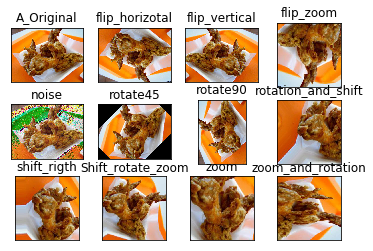
\includegraphics{ImageDataAugmaentation.png}
 	\caption{Anwendung von \textit{ImageDataAugmentation} }
 	\label{fig:ImageDataAugmentation}
 \end{figure}
 Neuronale Netzwerke können umso effektiver sein, je mehr Daten sie zur Verfügung haben. Es ist also mehr als wichtig über eine große Datenmenge zu verfügen\\
 
 
 Die Datenvermehrung ist eine Strategie, die es Praktikern ermöglicht, die Vielfalt der für Trainingsmodelle verfügbaren Daten deutlich zu erhöhen, ohne tatsächlich neue Daten zu sammeln.\\
 
 
 Selbst wenn die Daten von geringerer Qualität sind, können Algorithmen tatsächlich besser funktionieren, solange nützliche Daten durch das Modell aus dem ursprünglichen Datensatz extrahiert werden können.\\
 Der erste Ansatz ist die Generierung erweiterter Daten vor dem Training des Klassifikators.
 Aber bestehende Datensätze reichen vielleicht nicht aus, um ein tiefgehendes Lernnetzwerk zu trainieren. Aufbau eines leistungsfähigen Klassifikators aus unzureichenden Daten, Datenerweiterungsmethoden sind nützlich.\\
 Natürlich, wenn Sie viele Parameter haben, müssten Sie Ihrem Modell des maschinellen Lernens eine proportionale Anzahl von Beispielen zeigen, um eine gute Leistung zu erzielen. Außerdem ist die Anzahl der benötigten Parameter proportional zur Komplexität der Aufgabe, die Ihr Modell zu erfüllen hat.
 \\
 Naturellement, si vous avez beaucoup de paramètres, vous aurez besoin de montrer à votre modèle d'apprentissage machine un nombre proportionnel d'exemples, pour obtenir de bonnes performances. De plus, le nombre de paramètres dont vous avez besoin est proportionnel à la complexité de la tâche que votre modèle doit effectuer.\\
 Dies ist im Wesentlichen die Voraussetzung für die Datenvermehrung. Im realen Szenario haben wir möglicherweise einen Datensatz von Bildern, die unter einer begrenzten Anzahl von Bedingungen aufgenommen wurden. Unsere Zielanwendung kann jedoch unter einer Vielzahl von Bedingungen existieren, wie z.B. unterschiedliche Ausrichtung, Position, Maßstab, Helligkeit usw. Wir tragen diesen Situationen Rechnung, indem wir unser neuronales Netzwerk mit zusätzlichen synthetisch modifizierten Daten trainieren.\\
\subsubsection{Dropout}
Künstliche Neurone sind von biologischen Neuronen inspiriert, aber die Beiden unterscheidet sich sehr voneinander und einer der wichtigen Unterschiede ist, dass biologische Neuronen unvollkommene Maschine sind, die sehr oft nicht richtig funktioniert und das ist a priori nie den Fall bei  biologischen Neuronen. Wir könnten also glauben, dass \ac{KNN} die biologische übertreffen könnten.Es sei denn, dass diese Funktionsstörung von biologischen Neuronen nicht eine Schwäche ist, sondern eher eine Stärke ist.Eine der verblüffenden Entdeckungen in \ac{KI} Bereich ist, dass es wünschenswert ist, künstliche Neuronen von Zeit zu Zeit zu Fehlfunktionen zu bringen\cite{1}. \textcolor{red}{Jetzt können wir uns fragen, wie Dysfunktion von Neuronen die Performances neuronaler Netze verbessern kann}.Die zufällige Hinzufügen von Dysfunktionen in einer Schicht der \ac{KNN} wird \textit{Dropout} benannt und wurde von \cite[Geoffrey E. et al]{2} eingeführt.\\
\textbf{Wie funktioniert Dropout}\\
Genauer gesagt,Dropout bezeichnet die zeitliche zufällige Ausschaltung von Neuronen in einer (sichtbaren oder versteckten )Schicht der \ac{KNN}. Wie die Abbildung \ref{fig:Dropout} zeigt, wenn ein Neuron zufällig aus dem \ac{NN} entfernt wird, werden auch all seine ein- und ausgehenden Verbindungen entfernt.
In einer Dropout-Schicht wird ein Neuron \textit{n} unabhängig von andren Neuronen mit einer Wahrscheinlichkeit \textit{p} zurückgehalten, d.h \textit{n} wird mit einer Wahrscheinlichkeit von \textit{p} entfernt.Wie eine NN mit Dropout ausgewertet wird, wird in Abbildung \ref{fig:Dropout_} veranschaulicht.\cite{3}

	\begin{figure}[h]
	\begin{subfigure}{.5\textwidth}
		\centering
		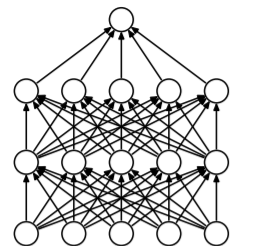
\includegraphics[scale=2, width=.8\linewidth, height=\linewidth]{dropout1.png}
			\caption{Standard neuronale Netze}
		\label{fig:dropout1}
	\end{subfigure}%
	\begin{subfigure}{.5\textwidth}
		\centering
		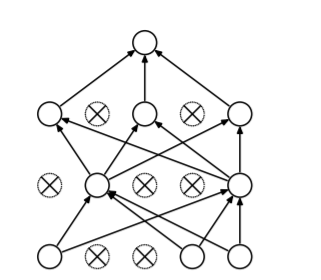
\includegraphics[width=.8\linewidth, height=\linewidth, scale=2]{dropout2.png}
		\caption{Netze nach Dropout}
		\label{fig:dropout2}
	\end{subfigure}
	\caption{Neuronales Netz mit Dropout \cite{3}}
	\label{fig:Dropout}
\end{figure}

\subsubsection{Vor- und Nachteile von Dropout}
\textbf{Automatische Erhöhung von Training Data }\\
Die Ausschaltung von Neuronen führt nicht nur dazu, dass jedes Neuron unabhängig von Anderen Mustern korrekt lernt, sondern auch dazu, dass neue Trainingsdaten automatisch erzeugt werden.\textcolor{red}{sollte ich auch die mathematische Formel Hinzufügen?}.Nehmen wir an, dass wir eine Dropout-Schicht $ D $  zwischen zwei \acsp{ConvL}  $ C1 $ und $ C2 $, so wird die Outputs $ O_{c1} $ von $ C1 $ zuerst von $ D $ umgewandelt, bevor sie in $ C2 $ einmünden.Die von $ D $ ausgeführte Transformation ergibt $ O_d = O'_{c1} +R $, wobei $ O'_{c1} $ Teilinformationen aus $ O_{c1} $  und $ R $  Informationen, die als Rauschen interpretieren werden können, bezeichnet. $ C2 $ soll also aus       $ O'_{c1} $ $ O_{c1} $ trotz $ R $ gut interpretieren können.
Für ein Netz mit $ n $ versteckten Einheiten, von denen jede fallen gelassen werden kann, haben wir durch Dropout $ 2^n $ mögliche Modelle. Das am Ende der Trainingszeit enthaltene Netz ist also eine durchschnittliche Approximation der $ 2^n $ mögliche verschiedene Modellen. In der Testphase wird das gesamte Netzwerk betrachtet und jede Aktivierung um einen Faktor p reduziert.
Durch die Anwendung von Dropout wird die Trainingszeit für jede Epoche geringer, aber die Anzahl der Iterationen, die für die Konvergenz notwendig sind, wird leider mindestens verdoppelt.
Dropout wendet also automatisch eine robuste Optimierung der neuronalen Netzwerkparameter an, die auch der Implementierung des \textit{Ockhams} Rasiermessers entspricht.

 \begin{figure}
	\centering
	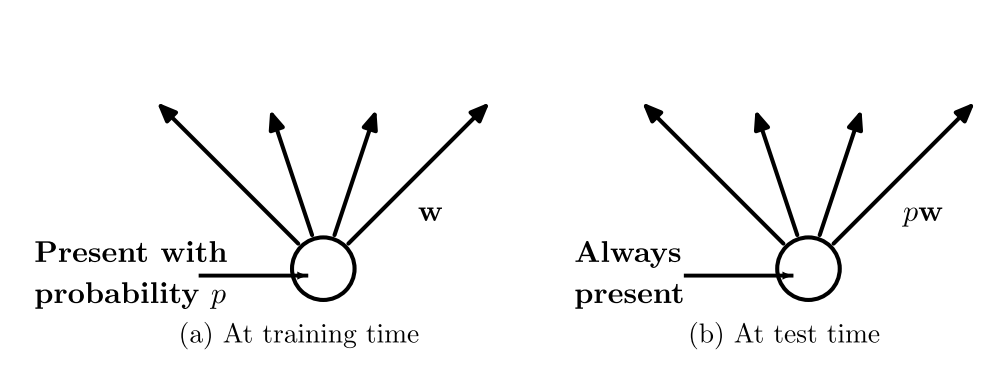
\includegraphics[width=\textwidth , height=0.3\linewidth]{dropout_}
	\caption{ \textbf{Links}: Ein Neuron zur Trainingszeit, die mit Wahrscheinlichkeit $ p $ vorhanden ist und mit Neuronen in der nächsten Schicht mit Gewichten w verbunden ist. 
		\textbf{Recht}: Zur Testzeit ist das Neuron immer vorhanden und die Gewichte werden mit $ p $ multipliziert. 
		Die Ausgabe zur Testzeit ist identisch mit der erwarteten Ausgabe zur Trainingszeit\cite{3}.}
	\label{fig:Dropout_}
\end{figure}
\subsubsection{Vergleich Ergebnisse}
\subsection{Batch-Normalisierung}
Das Training tiefer neuronaler Netze ist sehr kompliziert und ein Grund dafür ist zum Beispiel die Tatsache, dass die Parameter einer Schicht während des Trainings tiefer neuronaler Netze immer unter der Annahme, dass sich die Parameter anderer Schichten nicht ändern, aktualisiert werden und da alle Schichten während des Updates geändert werden, verfolgt das Optimierungsverfahren ein Minimum, das sich ständig bewegt. Ein anderer Grund dafür ist die ständigen Veränderungen im Laufe des Trainings in die Verteilung des Netzinputs, diese Veränderung wird von \cite{bactchnormalisation} als interne kovariate Verschiebung(\textit{Internal Covariate Shift}) genannt.Zur Lösung dieser Probleme schlagen \textit{LeCunn et al}\cite{LeCun} vor dem Training das Netzinput zu normalisieren. Aber dieser Ansatz bringt nicht so viel, wenn das \ac{NN} wirklich tief ist, denn nur der Netzinput profitiert von der Normalisierung und die kleinen Veränderungen in versteckte Schichten werden sich immer mehr verstärken, je tiefer man das Netz durchläuft. Mit der Ausbreitung tiefer \acsp{NN} dehnt Batch-Normalisierung(BN)\cite{bactchnormalisation} diese Idee der Datennormalisierung auf versteckte Schichten tiefer \acsp{NN} aus. Bei der BN werden die Eingaben in einem Netzwerk standardisiert, die entweder auf die Aktivierungen einer vorherigen Schicht oder auf direkte Eingaben angewendet wird, so standardisiert, dass der Mittelwert in der Nähe von null liegt und die Standardabweichung in der Nähe von eins liegt. Die BN wird über Mini-Batches und nicht über den gesamten Trainingssatz durchgeführt, daher enthalten wir nur Näherungen an tatsächliche Werte der Standardabweichung und des Mittelwerts über das Trainingssatzes, aber wir gewinnen an Geschwindigkeit und an Speicherplatzverbrauch.Die Gleichung \eqref{BNA} gibt die formale Beschreibung des BN Algorithmus an.
\begin{center}
	 Batch-Normalisierungstransformation, angewendet auf Aktivierung x über einen Mini-Batch
\end{center}
\begin{subequations}
	 \begin{align*}
		\textbf{Input:} & \text{  Werte von x über einer Mini-Batch: } B=\{x_{1...m}\}\\
		& \text{Lernbare Parameter  } \beta, \gamma \\
		\textbf{Output:} & \{ y_i = BN_{\beta, \gamma}(x_i)\}
	\end{align*}
	\begin{align}
		\text{Mini-Batch Mittelwert  : } &\mu_\beta=\frac{1}{m}\sum_{i = 1}^{m}x_i \\
		\text{ Mini-Batch Standardabweichung :} &\sigma_\beta^2=\frac{1}{m}\sum_{i = 1}^{m}(x_i- \mu_\beta)^2 \\
		 \text{Normalisierung:} & \widehat{x_i} = \frac{x_i - \mu_\beta}{\sqrt{\sigma_\beta^2 + \epsilon}} \\
		 \text{Skalierung und Verschiebung :} & {y_i} = \gamma\widehat{x_i} + \beta \equiv BN_{\gamma, \beta}
	\end{align}
	\label{BNA}
\end{subequations}

Wenn $\gamma = \sqrt{\sigma_\beta^2 + \epsilon}$ und $\beta = \mu_\beta $, bekommen wir die gleiche Verteilung wie vor der Batch-Normalisierung, d.h die Eingabe war also schon normalisiert. Interessanterweise kann das Netz während des Trainings eine bessere Verteilung als die erwünschte finden, denn $\gamma$ und $\beta$ sind lernbare Parameter.

 Durch die BN kann zum einen eine hohe Lernrate verwendet,was in tiefer \acsp{NN} ohne BN dazu führen kann, dass die Gradienten explodieren oder verschwinden und in schlechten lokalen Minima stecken bleiben.Die Verwendung einer höhere Lernrate ermöglicht einer schnellere Konvergenz.
 Zum anderen wird die interne kovariate Verschiebung geringer, was das Training beschleunigt, in einigen Fällen durch Halbierung der Epochen oder besser. Noch dazu wird das Netz durch die BN in gewissem Maße reguliert, daher wird die Verwendung von Dropout bzw. Regulierungstechnik reduziert oder sogar überflüssig und somit eine Verbesserung der Verallgemeinerungsgenauigkeit.



\section{Experiment}


\section{Abkürzungsverzeichnis}
\begin{acronym}[THIBAUT]
	\acro{KNN}{Künstliches neuronales Netz}
	\acro{CNN}{Convolutional Neural Network}
	\acro{KI}{Künstliche Intelligenz}
	\acro{NN}{neuronales Netz}
	\acro{ConvL}{Convolutional Layer}
	\acro{FCL}{Fully Connected Layer}
\end{acronym}
\bibliographystyle{agsm}
\begin{thebibliography}{lem00}
 \bibitem{1}
	P. Kerlirzin, and F. Vallet \href{ https://www.mitpressjournals.org/doi/abs/10.1162/neco.1993.5.3.473?journalCode=neco} {Robustness in Multilayer Perceptrons}
 \bibitem{2}
 	Geoffrey E. Hinton and Nitish Srivastava and Alex Krizhevsky and Ilya Sutskever and Ruslan R. Salakhutdinov \href{https://arxiv.org/abs/1207.0580}{Improving neural networks by preventing co-adaptation of feature detectors}
 \bibitem{3}
 	Srivastava, Hinton, Krizhevsky, Sutskever and Salakhutdinov \href{http://jmlr.org/papers/volume15/srivastava14a.old/srivastava14a.pdf}{Dropout: A Simple Way to Prevent Neural Networks from Overfitting}
\bibitem{4}
Ian Goodfellow, Yoshua Bengio, Aaron Courville
\href{https://www.amazon.com/Deep-Learning-Adaptive-Computation-Machine/dp/0262035618/ref=as_li_ss_tl?ieTF8&qid=1548018253&sr=8-3&keywords=deep+learning&linkCode=sl1&tag=inspiredalgor-20&linkId=49b3b1cce7e04bb3c9b99f2d878bf805&language=en_US}{Adaptive Computation and Machine Learning series} Page 342
 
 \bibitem{5}
	 Song Han, Huizi Mao, William J. Dally \href{https://arxiv.org/abs/1510.00149}{Deep Compression: Compressing Deep Neural Networks with Pruning, Trained Quantization and Huffman Coding}
 \bibitem{Automated Pruning}
      Franco Manessi, Alessandro Rozza, Simone Bianco, Paolo Napoletano, Raimondo Schettini \href{https://arxiv.org/abs/1712.01721}{Automated Pruning for Deep Neural Network Compression}
 \bibitem{7}
 	 Pavel Golik , Patrick Doetsch, Hermann Ney
 	\href{http://books.jackon.me/Cross-Entropy-vs-Squared-Error-Training-a-Theoretical-and-Experimental-Comparison.pdf}{Cross-Entropy vs. Squared Error Training:a Theoretical and Experimental Comparison}
 	
 \bibitem{8}
 	\href{http://www.neuronalesnetz.de/aktivitaet.html}{Neuronale Netze:Eine Einführung}
 	
 \bibitem{bactchnormalisation}
	Sergey Ioffe, Christian Szegedy
 	\href{https://arxiv.org/pdf/1502.03167.pdf}{Batch Normalization: Accelerating Deep Network Training b
 		y
 		Reducing Internal Covariate Shift}

	\bibitem{LearningRate}
		\href{https://en.wikipedia.org/wiki/Learning_rate}{Learning Rate}
	\bibitem{AdaGrad}
		John Duchi,Elad Hazan, Yoram Singer,
		\href{http://www.jmlr.org/papers/volume12/duchi11a/duchi11a.pdf}{Adaptive Subgradient Methods for
			Online Learning and Stochastic Optimization}
	\bibitem{adam}
		Diederik P. Kingma, Jimmy Ba
		\href{https://arxiv.org/abs/1412.6980}{Adam: A Method for Stochastic Optimization}
		
	\bibitem{quantization1}
		\href{https://nervanasystems.github.io/distiller/quantization.html}{Compressing Models:Quantization}
	\bibitem{quantizationYoni}
		Yoni Choukroun, Eli Kravchik, Fan Yang, Pavel Kisilev:
			\href{https://arxiv.org/abs/1902.06822}{Low-bit Quantization of Neural Networks for Efficient Inference}
	\bibitem{kneuron}
	wikipedia:\href{https://en.wikipedia.org/wiki/Artificial_neuron}{ Artificial neuron}
\end{thebibliography}

 
      
  % ggf. hier Tabelle mit Symbolen 
  % (kann auch auf das Inhaltsverzeichnis folgen)

\newpage
  
 \thispagestyle{empty}


\vspace*{8cm}


\section*{Erklärung}

Ich  versichere  wahrheitsgemäß,  die  Arbeit selbstständig verfasst,  alle  benutzten  Hilfsmittel  vollständig  und  genau  angegeben  und  alles kenntlich  gemacht  zu  haben,  was  aus  Arbeiten  anderer  unverändert  oder  mit  Abänderungen entnommen  wurde,  sowie die Satzung  der  Universität Augsburg  zur  Sicherung guter wissenschaftlicher Praxis in der jeweils gültigen Fassung beachtet zu haben.
\\[2ex] 

\noindent
Ort, den Datum\\[5ex]

% Unterschrift (handgeschrieben)



\end{document}

